\documentclass[../main.tex]{subfiles}
\graphicspath{{\subfix{../figures/}}}

\begin{document}
\chapter{安全基础技术实验}
\section{实验要求}
利用西普信息安全教育平台,从以下课程部分选取 2 个实验项目进行学习、
理解、设计和完成实验,书写所完成的内容。
%
\section{实验内容}
\begin{itemize}
  \item 密码学及应用
  \item 防火墙(*)
  \item 入侵检测系统
  \item 日志数据分析
  \item 数据库安全(*)
\end{itemize}
%
\section{防火墙}
%\documentclass[../main.tex]{subfiles}
\graphicspath{{\subfix{../figures/}}}

\begin{document}
\chapter{PGP 软件应用实验}
\section{实验介绍}
PGP 软件是一款优秀的个人安全防护软件。请安装并使用该软件的主要功能,
进行相关实验,验证 PGP 软件的可用性和有效性。
%
\section{实验内容}
密钥对的产生、公钥的导出导入、文件的加密、Email 的加密和签名、文件
的粉碎、虚拟磁盘加密、磁盘空间的粉碎等功能。
%
\section{报告内容}
按功能模块进行实验,并组织书写实验步骤与实验结果,
分别以不同小节给出。实验中请使用与学号、姓名等特征信息相关的实验数据,
体现相关实验是自己所完成的。
% 具体书写建议:每个部分先给出功能性简介描述;再针对每个功能模块进行实验操作,
% 给出相关步骤的文字描述,并附上相应步骤和结果贴图。贴图要大小合适,截图清晰。
% 建议按照以下几个部分书写,不能完成的部分就删除。
% 相关的技术原理等可以适当进行一些描述,以流程图、文字结合方式为佳。
\section{PGP 密钥对的产生与管理}
% 该部分包括个人密钥对的生成、公钥的导出与导入等。

\section{文件的加密与签名}
% 该部分包括使用 PGP 对文件、文件夹的加密、加密\&签名、签名等功能的操作。

\section{Email 的加密与签名}
% 该部分包括使用使用 Web 网页的 email 的书写、剪切、加密剪贴板内容、邮件发送、
% 邮件接收、复制密文邮件、PGP 解密剪贴板内容等步骤。

% 加密邮件可以 2 个同学以上合作完成一个实验,分别书写个人通信、操作的部分。

\section{文件的粉碎}
% 该部分包括使用 PGP 软件安全删除粉碎个人的隐私数据文档、文件夹等。

\section{虚拟磁盘的加密}
% 该部分包括使用 PGP 创建、加密生成一个加密的虚拟磁盘功能。

\section{磁盘空间的粉碎}
% 该部分包括使用 PGP 右击逻辑磁盘,实现对磁盘已删除内容的彻底清空操作。

%[1] 中 国 互 联 网 协 会 2006 年 第 一 次 反 垃 圾 邮 件 调 查 结 果
%[EOL].http://www.anti-spam.cnlShowArticle.php?id=2713
%[2] 曹麒麟,张千里.垃圾邮件与反垃圾邮件技术[M].北京:人民邮电出版社,2003.
%[3] 罗改龙.基于 SPI 的防火墙的研究与实现[硕士学位论文].武汉:武汉理工大学,2007
%[4] 周茜,赵明生.中文文本分类中的特征选择研究[J].中文信息学报,2003,Vol.18 No.3
\end{document}

%\subsection{实验目的-了解 iptables 中常见的一些相关名词和术语}
了解 iptables 中常见的一些相关名词和术语.
%
\subsection{实验原理}
\begin{itemize}
  \item iptables 是与 Linux 内核集成的 IP 信息包过滤系统。如果 Linux 系统连接
    到因特网或 LAN、服务器或连接 LAN 和因特网的代理服务器,则该系统有利于在
    Linux 系统上更好地控制 IP 信息包过滤和防火墙配置。
  \item 防火墙在做信息包过滤决定时,有一套遵循和组成的规则,这些规则存储在
    专用的信息包过滤表中,而这些表集成在 Linux 内核中。在信息包过滤表中,规
    则被分组放在我们所谓的链(chain)中。而 ``netfilter/iptables'' IP 信息包过
    滤系统是一款功能强大的工具,可用于添加、编辑和移除规则。
\end{itemize}
%
\subsubsection{iptables 防火墙}
\begin{itemize}
  \item Netfilter/Iptables(以下简称 iptables)是 Unix/Linux 自带的一款优秀
    且开放源码的完全基于包过滤的防火墙工具,它的功能十分强大,使用非常灵活,
    可以对流入和流出服务器的数据包进行很精细的控制。特别是它可以在一台非常
    低的硬件配置下跑得非常好。
  \item Netfilter/Iptables 的最大优点是它可以配置有状态的防火墙,这是老一
    辈 ipfwadm 和 ipchains 等以前的工具都无法提供的一种重要功能。Iptables 主
    要工作在 OSI 的二、三、四层,即数据链路层、网络层和传输层,如果重新编译
    内核,也可以支持 7 层控制。
  \item Iptables 防护墙由两个组件 netfilter 和 iptables 组成。
  \item netfilter 组件也称为内核空间(kernelspace),是内核的一部分,由一
    些信息包过滤表组成,这些表包含内核用来控制信息包过滤处理的规则集。
  \item iptables 组件是一种工具,也称为用户空间(userspace),它使插入、修
    改和除去信息包过滤表中的规则变得容易。
\end{itemize}
%
\subsubsection{iptables 名词和术语}
\begin{itemize}
  \item 容器:在 iptables 中,容器用来描述包含或者属于的关系。
  \item Netfilter:Netfilter 是表(tables)的容器。
  \item 表(tables):表(tables)是链的容器,即所有的链(chains)都属于对
    应的表(tables)。
  \item 链(chains):链(chains)是规则(policy)的容器。
  \item 规则(policy):规则(policy)是 iptables 一系列过滤信息的规范和具体方法。
\end{itemize}
我们可以用一个通俗易懂的例子表现这几个术语之间的关系。
\begin{table}[H]
  \begin{center}
    \begin{tabular}[c]{llll}
      \hline
      Netfilter & tables(表) & chains(链) & policy(规则) \\
      一栋楼 & 楼里的房间 & 房间里的柜子 & 柜子里的衣服摆放规则 \\
      \hline
    \end{tabular}
  \end{center}
\end{table}
%

%\subsection{实验目的-了解 iptables 中的表和链}
了解 iptables 中的表和链.
%
\subsection{实验原理}
\begin{itemize}
  \item Netfilter/iptables 是表(tables)的容器,iptables 包含 4 个表,分别是 filter、nat、mangel 和 raw。
  \item iptables 的表(tables)是链(chains)的容器,iptables 包含 5 个链,分别
    是 INPUT、OUTPUT、FORWARD、PREROUTING 和 POSTROUTING。
\end{itemize}
%
\subsection{实验原理}
\subsubsection{iptables 的表(tables)和链(chains)}
虽然 iptables 包含 4 个表,但是因为表 raw 在实际中很少或者基本上用不
到,所以默认情况下,iptables 根据功能和表的定义划分包含 3 个表:filter、
nat 和 mangel,其中,比较常用到的是 filter 和 nat。每个表又包含不同的操
作链(chains)。

下面的表格展示了表和链的对应关系,其中,1 表示有,0 则表示没有。
注意,所有链名必须大写。
\begin{table}[H]
  \begin{center}
    \begin{tabular}[c]{llllll}
      \hline
      表(tables)/链(chains) & INPUT & FORWARD & OUTPUT & PREROUTING & POSTROUTING \\
      \hline
      filter & 1 & 1 & 1 & 0 & 0 \\
      nat & 0 & 0 & 1 & 1 & 1 \\
      mangel & 1 & 1 & 1 & 1 & 1 \\
      \hline
    \end{tabular}
  \end{center}
\end{table}

下图展示了 filter 表和链 INPUT、FORWARD 和 OUTPUT 之间的对应关系。
\begin{figure}[H]
  \begin{center}
    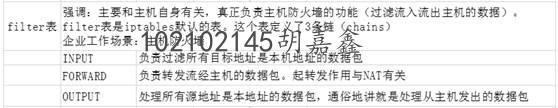
\includegraphics[width=0.40\textwidth]{2_3_1.jpeg}
  \end{center}
\end{figure}

下图展示了 nat 表和链 OUTPUT、PREROUTING 和 POSTROUTING 之间的对应关系。
\begin{figure}[H]
  \begin{center}
    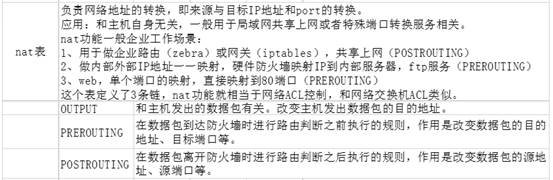
\includegraphics[width=0.40\textwidth]{2_3_2.jpeg}
  \end{center}
\end{figure}

Mangel 表主要负责修改数据包特殊的路由标记,如 TTL、TOS、MARK 等。由
于 mangel 表与特殊标记相关,一般情况下用不到这个表,这里就不做详细介绍
了。
%
\subsubsection{iptables 表和链工作的流程图}
下图清晰的描绘了 netfilter 对包的处理流程。
\begin{figure}[H]
  \begin{center}
    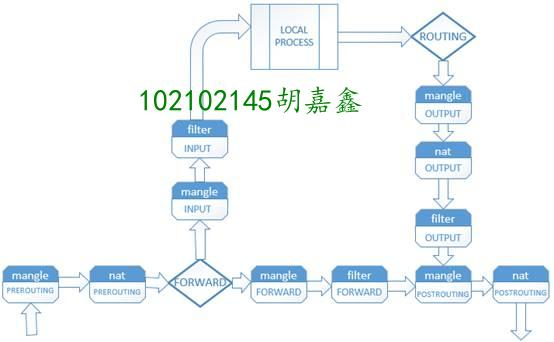
\includegraphics[width=0.40\textwidth]{2_3_3.jpeg}
  \end{center}
\end{figure}

为了更好的学习 iptables,可以将上图进行简化。
\begin{figure}[H]
  \begin{center}
    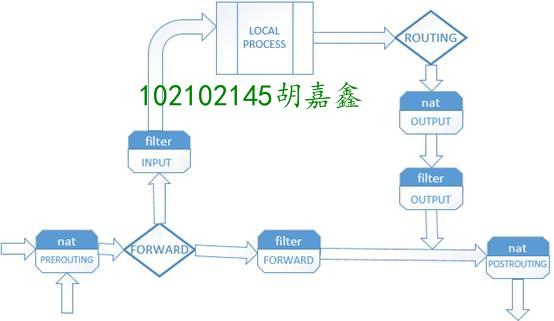
\includegraphics[width=0.40\textwidth]{2_3_4.jpeg}
  \end{center}
\end{figure}

上图可分为两个流程,上面的流程主要是 NAT 功能,在企业中常用于局域网
共享、将外部 IP 和端口映射为内部 IP 和端口等。下面的流程主要是 FILTER 功
能,即防火墙功能,企业中主要的应用是服务器防火墙。

%\subsection{实验目的-了解 iptables 常用的基本命令}
了解 iptables 常用的基本命令.
%
\subsection{实验原理}
iptables 是用来设置、维护和检查 Linux 内核的 IP 包过滤规则的。可以定
义不同的表,每个表都包含几个内部的链,也能包含用户自定义的链。每个链都
是一个规则列表,对对应的包进行匹配:每条规则指定应当如何处理与之相匹配
的包。这被称作 target(目标),也可以跳向同一个表内的用户定义的链。
%
\subsection{实验环境}
操作系统:CentOS 6.5
%
\subsection{实验步骤}
\subsubsection{查看 iptables 使用方法}
一般而言,我们学习某个软件的使用方法,除了在网上或者使用书籍进行
学习,最快捷有效的方式就是直接查看帮助。右键单击桌面,选择``在终端中打开''。
\begin{figure}[H]
  \begin{center}
    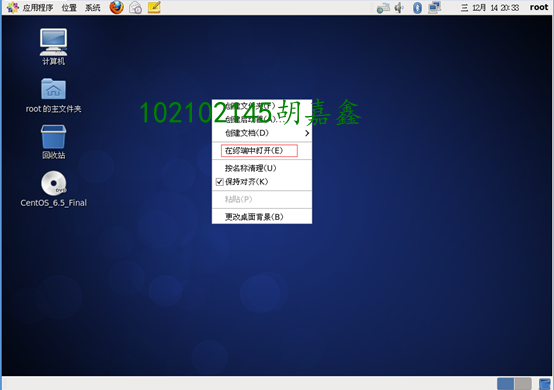
\includegraphics[width=0.50\textwidth]{2_4_1.png}
  \end{center}
\end{figure}

在终端中输入命令
\begin{minted}[bgcolor=bg]{sh}
iptables -h
\end{minted}
则会列出 iptables 的使用方法。
若想要看 iptables 更加详细的使用方法,可以使用命令
\begin{minted}[bgcolor=bg]{sh}
man iptables
\end{minted}
%
\subsubsection{iptables 基本命令}
iptables 命令的通用格式为:
\begin{minted}[bgcolor=bg,breaklines=true]{sh}
iptables [-t tables] COMMAND chain [-m matchname [per-match-options]] -j targetname [per-target-options]
\end{minted}
其中,tables 包括 filter、nat、mangel 和 raw,
chain 包括 INPUT、OUTPUT、FORWARD、PREROUTING 和 POSTROUTING。
当不指定表时,默认表为 filter。

iptables 命令的使用格式可用图表示如下。
\begin{figure}[H]
  \begin{center}
    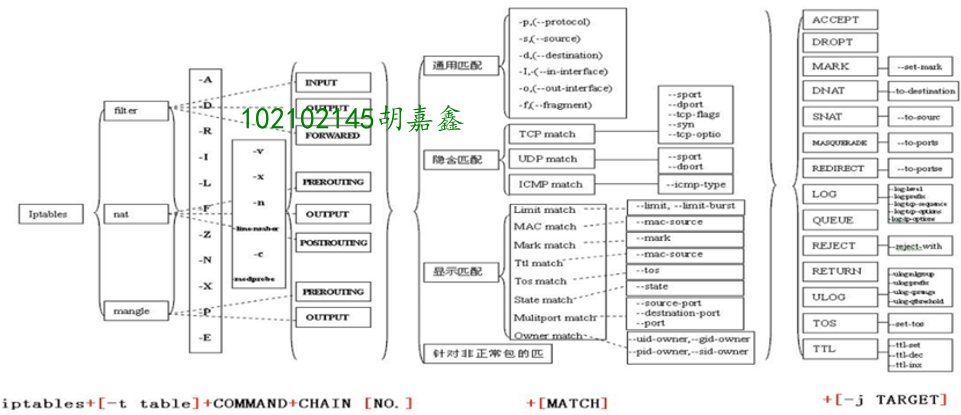
\includegraphics[width=0.50\textwidth]{2_4_2.png}
  \end{center}
\end{figure}

对上图进行简化。
\begin{figure}[H]
  \begin{center}
    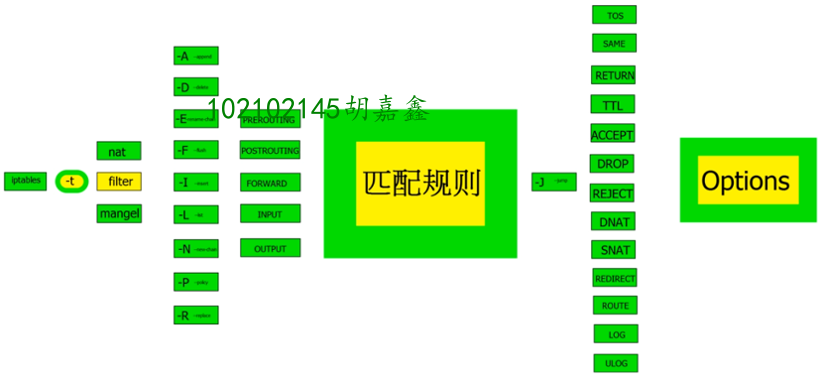
\includegraphics[width=0.50\textwidth]{2_4_3.png}
  \end{center}
\end{figure}

下面对 COMMAND 进行介绍。
\begin{enumerate}
  \item 常见用于链管理的参数有:
    \begin{itemize}
      \item \mintinline{sh}{-N}:new,自定义一条新的规则链
      \item \mintinline{sh}{-X}:delete/drop, 删除自定义的规则链,指明名字删除一个,不指明将删除多个
      \item \mintinline{sh}{-P}:policy,设置默认策略,指明是黑名单还是白名单,对于 filter 表中的链
        而言,其默认策略有 ACCEPT(接受)、DROP(丢弃)和 REJECT(拒绝)
      \item \mintinline{sh}{-E}:重命名自定义链,引用计数不为 0 的自定义链,不能被重命名或者删除
    \end{itemize}
  \item 常见的用于规则管理的参数有:
    \begin{itemize}
      \item \mintinline{sh}{-A}:append,追加规则
      \item \mintinline{sh}{-I}:insert,插入规则,需要指明位置,省略时表示第一条
      \item \mintinline{sh}{-D}:delete,删除规则,指明规则号删除或者指明规则本身
      \item \mintinline{sh}{-R}:replace,替换指定链上的指定规则,指明替换号或者指明替换规则本身
      \item \mintinline{sh}{-F}:flush,清空指定的规则链,指明链,即清空指定链上的规则;不指明链,
        即清空所有链上的规则
      \item \mintinline{sh}{-Z}:zero, 置零,匹配到的报文个数或者匹配到的所有报文的大小之和(字节数)
    \end{itemize}
  \item 查看信息的常用参数有:
    \begin{itemize}
      \item \mintinline{sh}{-L}:必选,list,列出指定链上的所有规则,下面的几个为附加子参数
      \item \mintinline{sh}{-n}:numberic,以数据格式显示地址和端口
      \item \mintinline{sh}{-v}:verbose,详细信息,vv 或者 vvv(v 的个数越多越详细)
      \item \mintinline{sh}{-x}:exactly(精确的),显示计数器结果的精确值
      \item \mintinline{sh}{--line-numbers}:显示规则的序号
    \end{itemize}
\end{enumerate}

下面对匹配条件进行介绍。
\begin{enumerate}
  \item  基本匹配条件:无需加载任何模块,由 iptables/netfilter 自行提供
    \begin{itemize}
      \item \mintinline{sh}{-s,--source address[/mask][,...]}:检查报文中源 IP 地址, 是否符合此处指
        定的地址或范围
      \item \mintinline{sh}{-d,--destination address[/mask][,...]}:检查报文中的目标 IP 地址,是否符
        合此处指定的地址或范围
      \item \mintinline{sh}{-p,--protocol protocol}:表明在传输层应用的协议,其可以有 tcp,udp,udplite,
        icmp,icmpv6,esp,ah,sctp,mh 或者 all(包括 tcp、udp 和 icmp 3 个)
      \item \mintinline{sh}{-i,--in-interface name}:
        只能应用于数据报文流入的接口,作用于链 INPUT,FORWARD 和 PREROUTING
      \item \mintinline{sh}{-o,--out-interface name}:只能应用于数据报文流出的接口, 作用于链 OUTPUT,
        FORWARD 和 POSTROUTING
    \end{itemize}
  \item  隐匿扩展:不需要手动加载扩展模块,因为它们是对协议的扩展,所以但凡使
    用 \mintinline{sh}{-p} 指明了协议,就表示已经指明了要扩展的模块
    \begin{itemize}
      \item tcp 协议:
        \begin{enumerate}
          \item \mintinline{sh}{--source-port,--sport port[:port]}:匹配报文的源端口,可以是端口范围
          \item \mintinline{sh}{--destination-port,--dport port[:port]}:匹配报文的目标端口,可以是端口范围
          \item \mintinline{sh}{--tcp-flags mask comp}:mask 为必须要检查的标识位,必须以逗号分隔;comp
            必须为 1 的标识位,必须以逗号分隔
          \item \mintinline{sh}{--syn}:匹配第一次握手
        \end{enumerate}
      \item udp 协议:
        \begin{enumerate}
          \item \mintinline{sh}{--source-port,--sport port[:port]}: 匹配报文的源端口,可以是端口范围
          \item \mintinline{sh}{--destination-port,--dport port[:port]}:匹配报文的目标端口,可以是端口范围
        \end{enumerate}
      \item icmp 协议:\mintinline{sh}{--icmp {type[/code] | typename}}
    \end{itemize}
  \item  显示扩展:必须使用\mintinline{sh}{-m} 选项手动加载模块,
    其扩展模块路径为: \mintinline{sh}{/lib64/xtables},
    其中大写的为目标扩展,小写的为规则扩展。
  \item multiport 扩展:以离散方式定义多端口匹配,但最多指定 15 个端口
    \begin{enumerate}
      \item \mintinline{sh}{--source-ports,--sports port[,port|,port:port]}:指定多个源端口
      \item \mintinline{sh}{--destination-ports,--dports port[,port|,port:port]}:指定多个源端口
      \item \mintinline{sh}{--ports port[,port|,port:port]}:指定多个目标及源端口
    \end{enumerate}
  \item iprange 扩展:指明连续的(不过一般不能是整个网络)ip 地址范围
    \begin{enumerate}
      \item \mintinline{sh}{--src-range from[-to]}:源 IP 地址
      \item \mintinline{sh}{--dst-range from[-to]}:目标 IP 地址
    \end{enumerate}
  \item connlimit 扩展:对每客户端 IP 做并发连接数量匹配
    \begin{enumerate}
      \item \mintinline{sh}{--connlimit-upto n}:当现在的连接数量低于或等于这个数量(n),就匹配
      \item \mintinline{sh}{--connlimit-above n}:当现有的连接数量大于这个数量, 就匹配
    \end{enumerate}
  \item limit 扩展:基于收发报文的速率做匹配
    \begin{enumerate}
      \item \mintinline{sh}{--limit rate [/second|/minute|/hour]}:平均速率
      \item \mintinline{sh}{--limit-burst NUMBER}:峰值数量,默认 5 个
    \end{enumerate}
  \item state 扩展:根据连接追踪机制,查检连接的状态,
    跟 TCP 没有关系,是内核中 netfilter 实现,
    能实现 tcp,udp,icmp 的连接追踪,
    内核会记录每一个连接(放置在内存中),谁通过什么协议访问什么服务,
    访问的时间,这种机制被称之为 conntrack 机制。
    也正是有了 state 扩展,iptables 成为了有连接追踪的防火墙,
    安全性更高。是由 state 扩展提供,
    库文件为 \mintinline{sh}{ibxt_conntrack.so}。
    追踪连接功能在内核的内存空间中,把出去和进来的连接通过模板建立关联关系.
    追踪本机的请求和响应之间的关系,状态如下几种:
    \begin{enumerate}
      \item NEW:新发起的请求
      \item ESTABLISHED:new 状态之后,连接追踪模板中为其建立的条目失效之前期间内所有的通信状态
      \item RELATED:相关的连接,如 FTP 协议中的命令连接与数据连接之间的关系
      \item INVALID:无效的连接,如 tcp 状态全为 1 或者全为 0 的连接
      \item UNTRACKED:未进行追踪的连接
    \end{enumerate}
    调整连接追踪功能所容纳的最大连接数量:
    \begin{minted}[bgcolor=bg]{sh}
    /proc/sys/net/nf_conntrack_max
    \end{minted}
    已经追踪到的并记录下来的连接:
    \begin{minted}[bgcolor=bg]{sh}
    /porc/net/nf_conntrack
    \end{minted}
    不同协议的连接追踪状态时长(可修改):
    \begin{minted}[bgcolor=bg]{sh}
    /proc/sys/net/netfilter
    \end{minted}
    \mintinline{sh}{--state STATE}:
    多个 state 可以使用逗号分隔.
    iptables 的连接追踪表最大容量为
    \begin{minted}[bgcolor=bg]{sh}
    cat /proc/sys/ipv4/ip_conntrack_max
    \end{minted}
    链接达到各种状态的超时后,会从表中删除,
    当模板满载时,后续的链接可能会超时,可以有如下两种解决方法
    (但加大 max 值, 也会加大内存的压力)
    \begin{enumerate}
      \item 修改 max 的内核参数:
        \begin{minted}[bgcolor=bg]{sh}
        vim /etc/sysctl.conf
        \end{minted}
      \item 降低 \mintinline{sh}{nf_conntrack timout} 时间:
        \begin{minted}[bgcolor=bg]{sh}
        vim /etc/sysctl.conf
        \end{minted}
        放行被动模式的 ftp 服务,
        需手动加载 \mintinline{sh}{nf_conntrack_ftp}:
        \begin{minted}[bgcolor=bg]{sh}
        modprobe nf_conntrack_ftp
        \end{minted}
    \end{enumerate}
\end{enumerate}
%
target 的分类:
\begin{enumerate}
  \item ACCEPT:接受
  \item DROP:丢弃
  \item REJECT:拒绝
  \item RETURN:返回调用链
  \item REDIRECT:端口重定向
  \item LOG:记录日志,\mintinline{sh}{--log-level LEVEL} 用于设置日志的等级,
    \mintinline{sh}{--log-prefix PFREFIX} 用于设置日志的提示语句的前缀
  \item MASK:做防火墙标记
  \item DNAT:目标地址转换
  \item SNAT:源地址转换
  \item MASQUERADE:地址伪装
\end{enumerate}

%\subsection{实验目的-熟悉 iptables 的表链操作}
熟悉 iptables 的表链操作.
%
\subsection{实验原理}
通过 iptables 命令对防火墙 iptables 的表链进行相关操作(因环境策略不
同,表链会有所不同),如查看、添加、删除、修改等等。
%
\subsection{实验环境}
操作系统: CentOS 6.5
%
\subsection{实验步骤}
\subsubsection{Iptables 链操作}
查看 CentOS 6.5 中防火墙 iptables 的表名(因环境策略不同,表会有所不
同)。
在终端输入命令
\begin{minted}[bgcolor=bg,breaklines=true]{sh}
cat /proc/net/ip_tables_names
\end{minted}
若无结果,请查看是否开启服务。
可执行
\begin{minted}[bgcolor=bg,breaklines=true]{sh}
service iptables restart
\end{minted}
重启服务后再次执行,可以看到 iptables 包含 4 张表,
分别是 mangle、raw、filter 和 nat
(默认只有 filter 表,如果之前有对其他表进行过相关操作,才会有其他表)。
\begin{figure}[H]
  \begin{center}
    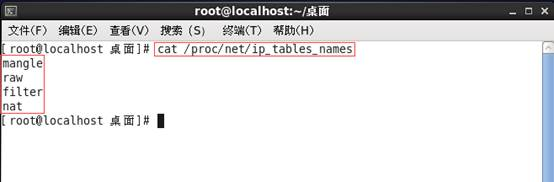
\includegraphics[width=0.40\textwidth]{2_5_1.jpeg}
  \end{center}
\end{figure}

在终端输入命令
\begin{minted}[bgcolor=bg,breaklines=true]{sh}
iptables -t filter -L
\end{minted}
查看表 filter 中的链及其链中的规则。
\mintinline{sh}{-t filter} 指定表 filter,也可不加,不加时默认表 filter。可知
表 filter 有 3 条链:
INPUT、FORWARD 和 OUTPUT,这 3 条链的默认规则都为 ACCEPT。
\begin{figure}[H]
  \begin{center}
    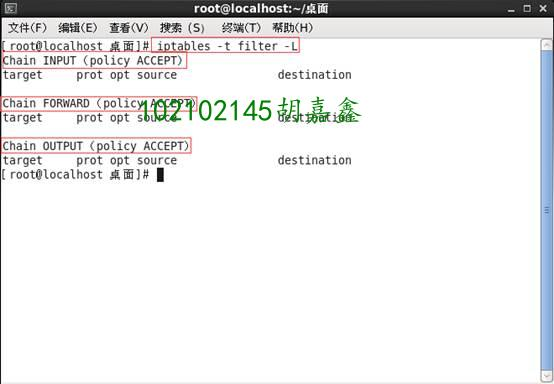
\includegraphics[width=0.40\textwidth]{2_5_2.jpeg}
  \end{center}
\end{figure}

若要查看某条链上的规则,在 \mintinline{sh}{-L} 参数后指明链名。
例如在终端输入命令
\begin{minted}[bgcolor=bg,breaklines=true]{sh}
iptables -L FORWARD
\end{minted}
查看表 filter 中链 FORWARD 上的规则。
\begin{figure}[H]
  \begin{center}
    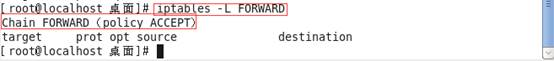
\includegraphics[width=0.40\textwidth]{2_5_3.jpeg}
  \end{center}
\end{figure}

在终端输入命令
\begin{minted}[bgcolor=bg,breaklines=true]{sh}
iptables -t nat –L
\end{minted}
查看表 nat 中的链及其链中的规则。
可知表 nat 有 3 条链:PREROUTING、POSTROUTING 和 OUTPUT,
这 3 条链的默认规则都为 ACCEPT。
\begin{figure}[H]
  \begin{center}
    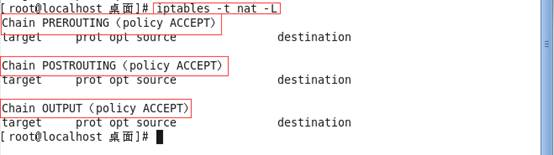
\includegraphics[width=0.40\textwidth]{2_5_4.jpeg}
  \end{center}
\end{figure}

在终端输入命令
\begin{minted}[bgcolor=bg,breaklines=true]{sh}
iptables -t mangle –L
\end{minted}
查看表 mangle 中的链及其链中的规则。
可知表 nat 有 5 条链:PREROUTING、INPUT、FORWARD、OUTPUT 和 POSTROUTING,
这 5 条链的默认规则都为 ACCEPT。
\begin{figure}[H]
  \begin{center}
    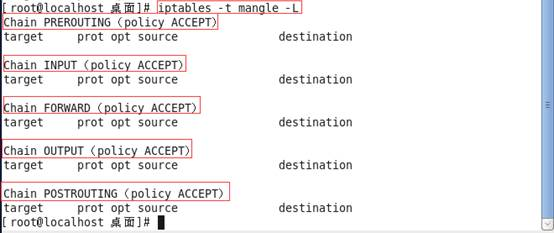
\includegraphics[width=0.40\textwidth]{2_5_5.jpeg}
  \end{center}
\end{figure}

在终端输入命令
\begin{minted}[bgcolor=bg,breaklines=true]{sh}
iptables -t raw –L
\end{minted}
查看表 nat 中的链及其链中的规则。
可知表 raw 有 2 条链:PREROUTING 和 OUTPUT,
这 2 条链的默认规则都为 ACCEPT。
\begin{figure}[H]
  \begin{center}
    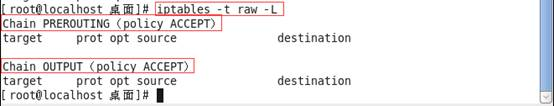
\includegraphics[width=0.40\textwidth]{2_5_6.jpeg}
  \end{center}
\end{figure}

在终端输入命令
\begin{minted}[bgcolor=bg,breaklines=true]{sh}
cat /etc/sysconfig/iptables
\end{minted}
(因环境策略不同,表中链及链中规则会有所不同),
查看防火墙配置文件,可以查看到 iptables 所有表中的链及其链中规则
(默认只有 filter 表,如果之前有对其他表进行过相关操作,才会有其他表)。
\begin{figure}[H]
  \begin{center}
    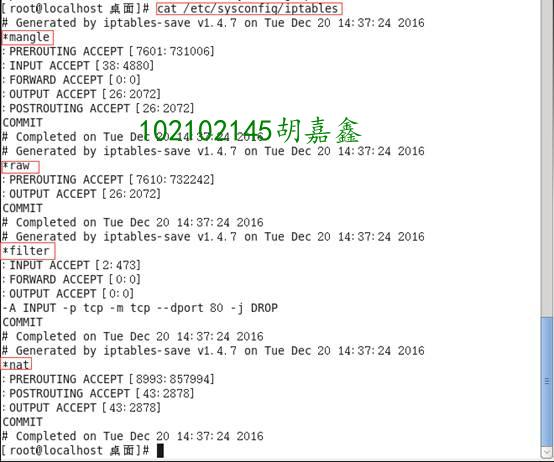
\includegraphics[width=0.40\textwidth]{2_5_7.jpeg}
  \end{center}
\end{figure}

这 4 张表 5 条链中的规则 target 为目标;prot 为协议;opt 为 option,
选项;source 为源地址,destination 为目的地址。在终端输入命令
\begin{minted}[bgcolor=bg,breaklines=true]{sh}
cat /proc/net/ip_tables_targets
\end{minted}
查看 iptables 中的 targets。
\begin{figure}[H]
  \begin{center}
    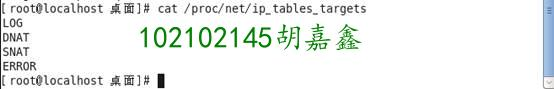
\includegraphics[width=0.40\textwidth]{2_5_8.jpeg}
  \end{center}
\end{figure}

在终端输入命令
\begin{minted}[bgcolor=bg,breaklines=true]{sh}
iptables -N simpleware1
\end{minted}
在表 filter 中添加一条名为 simpleware1 的新链。
这里没有使用 \mintinline{sh}{-t} 指定表,
默认是 filter 表,还可用 \mintinline{sh}{-t nat/mangle/raw}
在指定的表中添加新的链。再使用
\begin{minted}[bgcolor=bg,breaklines=true]{sh}
iptables -L
\end{minted}
进行查看。
\begin{figure}[H]
  \begin{center}
    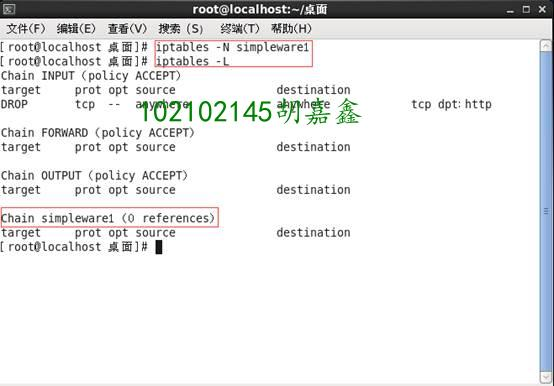
\includegraphics[width=0.40\textwidth]{2_5_9.jpeg}
  \end{center}
\end{figure}

使用上一步的方法继续在表 filter 中添加两条新链
simpleware2 和 simpleware3。
\begin{figure}[H]
  \begin{center}
    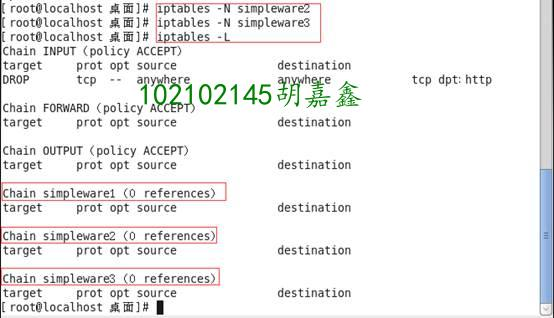
\includegraphics[width=0.40\textwidth]{2_5_10.jpeg}
  \end{center}
\end{figure}

若想删除某条自定义的链,使用 \mintinline{sh}{-X} 参数。
在终端输入命令
\begin{minted}[bgcolor=bg,breaklines=true]{sh}
iptables -X simpleware1
\end{minted}
删除表 filter 中自定义的链 simpleware1。
\begin{figure}[H]
  \begin{center}
    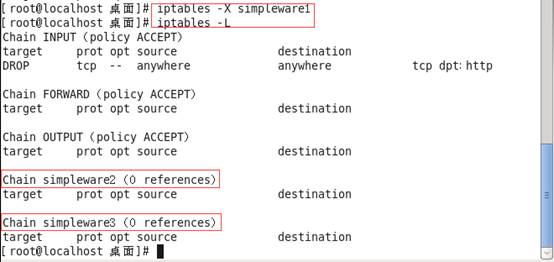
\includegraphics[width=0.40\textwidth]{2_5_11.jpeg}
  \end{center}
\end{figure}

在终端输入命令
\begin{minted}[bgcolor=bg,breaklines=true]{sh}
iptables -X
\end{minted}
直接删除表 filter 中所有自定义的链。
\begin{figure}[H]
  \begin{center}
    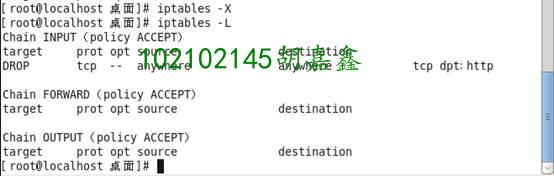
\includegraphics[width=0.40\textwidth]{2_5_12.jpeg}
  \end{center}
\end{figure}

可以使用 \mintinline{sh}{-P} 参数修改某条链的默认规则。
例如在终端输入命令
\begin{minted}[bgcolor=bg,breaklines=true]{sh}
iptables -P INPUT DROP
\end{minted}
将表 filter 中的链 INPUT 的默认规则改为 DROP。
\begin{figure}[H]
  \begin{center}
    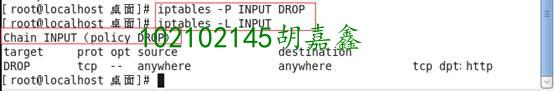
\includegraphics[width=0.40\textwidth]{2_5_13.jpeg}
  \end{center}
\end{figure}

在终端输入如下命令,分别在filter表的3条链上添加一条防火墙规则。
\begin{figure}[H]
  \begin{center}
    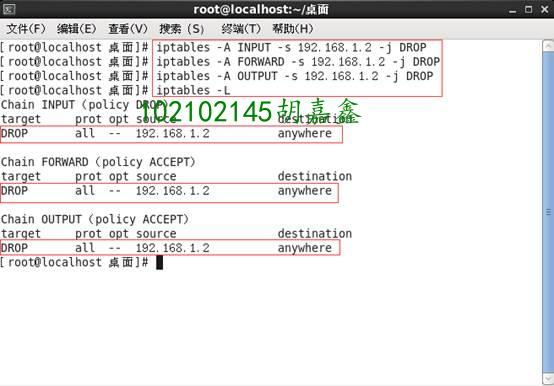
\includegraphics[width=0.40\textwidth]{2_5_14.jpeg}
  \end{center}
\end{figure}

在终端输入命令
\begin{minted}[bgcolor=bg,breaklines=true]{sh}
iptables -F INPUT
\end{minted}
清空 filter 表中 INPUT 链上的所有规则。
\begin{figure}[H]
  \begin{center}
    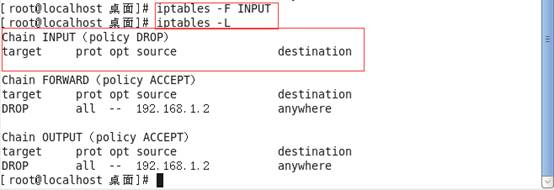
\includegraphics[width=0.40\textwidth]{2_5_15.jpeg}
  \end{center}
\end{figure}

在终端输入命令
\begin{minted}[bgcolor=bg,breaklines=true]{sh}
iptables -F
\end{minted}
不指明链名时,删除表 filter 中所有链上的规则。
\begin{figure}[H]
  \begin{center}
    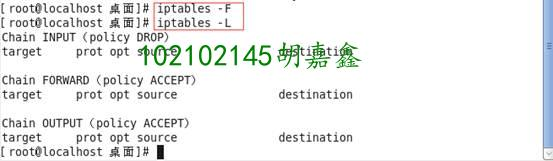
\includegraphics[width=0.40\textwidth]{2_5_16.jpeg}
  \end{center}
\end{figure}

\subsection{实验目的-配置 iptables 禁止访问 ftp 服务}
通过配置 iptables 防火墙禁止访问 ftp 服务
%
\subsection{实验原理}
\begin{enumerate}
  \item Iptables 防火墙在做信息包过滤决定时,有一套遵循和组成的规则,这些规
    则存储在专用的信息包过滤表中,而这些表集成在 Linux 内核中。在信息包过滤
    表中,规则被分组放在我们所谓的链(chain)中。而 \texttt{netfilter/iptables} IP
    信息包过滤系统是一款功能强大的工具,可用于添加、编辑和移除规则。
  \item FTP 是 File Transfer Protocol(文件传输协议)的英文简称,而中文简称
    为“文传协议”。用于 Internet 上的控制文件的双向传输。同时,它也是一个
    应用程序(Application)。基于不同的操作系统有不同的 FTP 应用程序,而所
    有这些应用程序都遵守同一种协议以传输文件。在 FTP 的使用当中,用户经常遇
    到两个概念:"下载"(Download)和"上传"(Upload)。"下载"文件就是从远程
    主机拷贝文件至自己的计算机上;"上传"文件就是将文件从自己的计算机中拷贝
    至远程主机上。用 Internet 语言来说,用户可通过客户机程序向(从)远程主
    机上传(下载)文件。
\end{enumerate}
%
\subsection{实验环境}
操作系统:
\begin{itemize}
  \item Windows 7
  \item Windows server 2003
  \item CentOS 6.5
  \item CentOS 6.5
\end{itemize}
%
\subsection{实验步骤}
\subsubsection{在当前环境下内外网均可连接 ftp 服务}
打开 Windows 7 的 cmd,
输入
\begin{minted}[bgcolor=bg,breaklines=true]{sh}
ftp 10.0.0.2
\end{minted}
输入用户名 \texttt{ftp},密码 \texttt{123456},登录成功。
%\begin{figure}[H]
  %\begin{center}
    %\includegraphics[width=0.50\textwidth]{}
  %\end{center}
%\end{figure}

打开 Windows server 2003 的 cmd,
输入
\begin{minted}[bgcolor=bg,breaklines=true]{sh}
ftp 10.0.0.2
\end{minted}
输入用户名 \texttt{ftp},
密码 \texttt{123456},登录成功。
%\begin{figure}[H]
  %\begin{center}
    %\includegraphics[width=0.50\textwidth]{}
  %\end{center}
%\end{figure}
%
\subsubsection{配置 iptables ,禁止内外网访问 ftp 服务}
在防火墙 CentOS 6.5 的终端输入如下命令,清空防火墙规则。
\begin{minted}[bgcolor=bg,breaklines=true]{sh}
iptables -F
iptables -X
iptables -Z
iptables -L -n --line-numbers
\end{minted}
%\begin{figure}[H]
  %\begin{center}
    %\includegraphics[width=0.50\textwidth]{}
  %\end{center}
%\end{figure}

配置防火墙,禁止内外网访问 ftp 服务。
因为这里我们使用 CentOS 6.5 充当防火墙,数据会在网卡之间进行转发,
所以我们这里对 filter 表的链 FORWARD 进行配置。
在终端输入如下命令,在转发的数据包中,如果目标端口为 21,则
将该数据包丢弃。
\begin{minted}[bgcolor=bg,breaklines=true]{sh}
iptables -t filter -A FORWARD -p tcp --dport 21 -j DROP
\end{minted}
%\begin{figure}[H]
  %\begin{center}
    %\includegraphics[width=0.50\textwidth]{}
  %\end{center}
%\end{figure}

在终端输入如下命令,将添加的规则保存到 iptables 配置文件中,重启防火墙,
查看防火墙规则。
%\begin{figure}[H]
  %\begin{center}
    %\includegraphics[width=0.50\textwidth]{}
  %\end{center}
%\end{figure}

此时在 Windows 7 的 cmd 上,输入
\begin{minted}[bgcolor=bg,breaklines=true]{sh}
ftp 10.0.0.2
\end{minted}
已经不能连接 ftp 服务了。
%\begin{figure}[H]
  %\begin{center}
    %\includegraphics[width=0.50\textwidth]{}
  %\end{center}
%\end{figure}

同样在 Windows server 2003 的 cmd 上,输入
\begin{minted}[bgcolor=bg,breaklines=true]{sh}
ftp 10.0.0.2
\end{minted}
也已经不能连接 ftp 服务了。
%\begin{figure}[H]
  %\begin{center}
    %\includegraphics[width=0.50\textwidth]{}
  %\end{center}
%\end{figure}
%

%\subsection{实验目的-配置 iptables 按网段访问 ftp 服务}
通过配置 iptables 防火墙来按网段访问 ftp 服务.
%
\subsection{实验原理}
Iptables 防火墙在做信息包过滤决定时,有一套遵循和组成的规则,这些规
则存储在专用的信息包过滤表中,而这些表集成在 Linux 内核中。在信息包过滤
表中,规则被分组放在我们所谓的链(chain)中。而 \texttt{netfilter/iptables} IP
信息包过滤系统是一款功能强大的工具,可用于添加、编辑和移除规则。
%
\subsection{实验环境}
操作系统:
\begin{itemize}
  \item Windows 7
  \item Windows server 2003
  \item CentOS 6.5
  \item CentOS 6.5
\end{itemize}
%
\subsection{实验步骤}
\subsubsection{在当前环境下内外网均可连接 ftp 服务}
打开 Windows 7 的 cmd,
输入
\begin{minted}[bgcolor=bg,breaklines=true]{sh}
ftp 10.0.0.2
\end{minted}
输入用户名 \texttt{ftp},密码 \texttt{123456},登录成功。
\begin{figure}[H]
  \begin{center}
    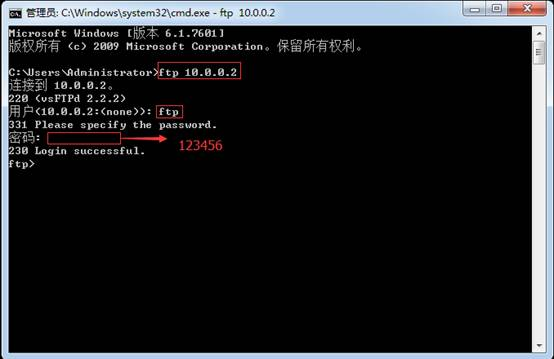
\includegraphics[width=0.40\textwidth]{2_7_1.jpeg}
  \end{center}
\end{figure}

打开 Windows server 2003 的 cmd,
输入
\begin{minted}[bgcolor=bg,breaklines=true]{sh}
ftp 10.0.0.2
\end{minted}
输入用户名 \texttt{ftp},
密码 \texttt{123456},登录成功。
\begin{figure}[H]
  \begin{center}
    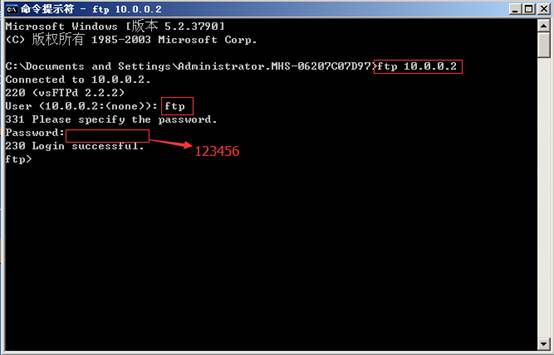
\includegraphics[width=0.40\textwidth]{2_7_2.jpeg}
  \end{center}
\end{figure}
%
\subsubsection{配置 iptables,按网段访问 ftp 服务}
这里以 Windows server 2003 能够访问 ftp 服务,
而 Windows 7 不能访问 ftp 服务为例.

在防火墙 CentOS 6.5 的终端输入如下命令,清空防火墙规则。
\begin{minted}[bgcolor=bg,breaklines=true]{sh}
iptables -F
iptables -X
iptables -Z
iptables -L -n --line-numbers
\end{minted}
\begin{figure}[H]
  \begin{center}
    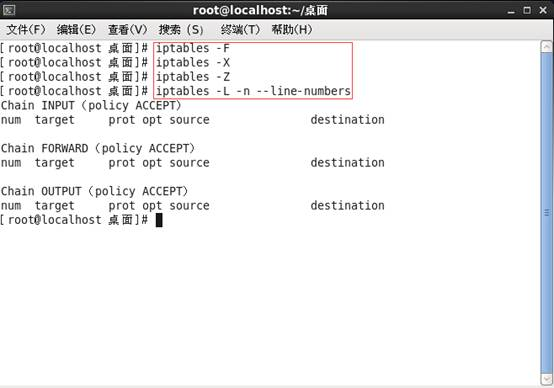
\includegraphics[width=0.40\textwidth]{2_7_3.jpeg}
  \end{center}
\end{figure}

配置防火墙,按网段访问 ftp 服务。在终输入如下命令,在转发的数据包
中,如果源地址为 \texttt{192.168.1.0/24},
目标端口为 21,则将该数据包丢弃,同时
允许源地址为 \texttt{20.0.0.2/24},
目标端口为 21 的数据包通过,这一条防火墙规则可加可不加。
\begin{minted}[bgcolor=bg,breaklines=true]{sh}
iptables -t filter -A FORWARD -s 192.168.1.0/24 -p tcp --dport 21 -j DROP
iptables -t filter -A FORWARD -s 20.0.0.0/24 -p tcp --dport 21 -j ACCEPT
/etc/init.d/iptables save
/etc/init.d/iptables restart
cat /etc/sysconfig/iptables
\end{minted}
\begin{figure}[H]
  \begin{center}
    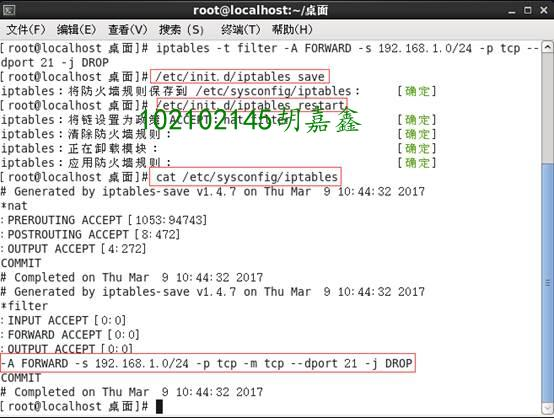
\includegraphics[width=0.40\textwidth]{2_7_4.jpeg}
  \end{center}
\end{figure}

此时在 Windows 7 的 cmd 上,
输入
\begin{minted}[bgcolor=bg,breaklines=true]{sh}
ftp 10.0.0.2
\end{minted}
已经不能连接 ftp 服务了。
\begin{figure}[H]
  \begin{center}
    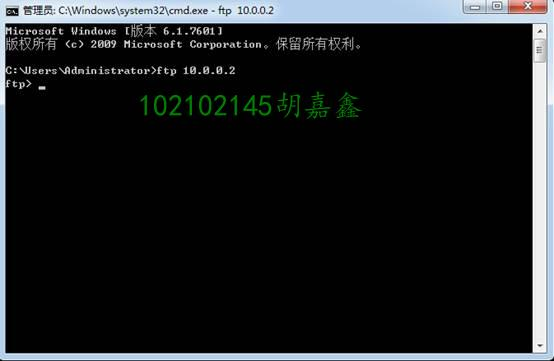
\includegraphics[width=0.40\textwidth]{2_7_5.jpeg}
  \end{center}
\end{figure}

但在 Windows server 2003 的 cmd 上,
输入
\begin{minted}[bgcolor=bg,breaklines=true]{sh}
ftp 10.0.0.2
\end{minted}
可以继续连接 ftp 服务。
\begin{figure}[H]
  \begin{center}
    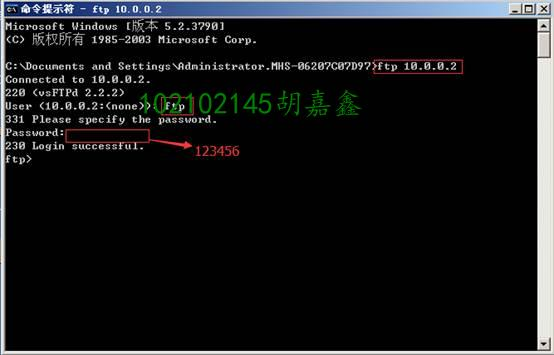
\includegraphics[width=0.40\textwidth]{2_7_6.jpeg}
  \end{center}
\end{figure}
%

%\subsection{实验目的-通过编写脚本配置防火墙}
通过编写脚本配置防火墙.
%
\subsection{实验原理}
编写脚本,执行脚本,完成防火墙的配置.
%
\subsection{实验环境}
操作系统: CentOS 6.5
%
\subsection{实验步骤}
\subsubsection{使用脚本配置防火墙}
在防火墙 CentOS 6.5 桌面新建 \texttt{firewall.sh},
在终端输入命令
\begin{minted}[bgcolor=bg,breaklines=true]{sh}
vi firewall.sh。
\end{minted}
%\begin{figure}[H]
  %\begin{center}
    %\includegraphics[width=0.50\textwidth]{}
  %\end{center}
%\end{figure}

编辑脚本 \texttt{firewall.sh},文件内容如下。
\begin{minted}[bgcolor=bg,breaklines=true]{sh}
#!/bin/bash
IPT="/sbin/iptables"
#Remove any existing rules
$IPT -F
$IPT -X
$IPT -Z
#setting for loopback interface
$IPT -t filter -A INPUT -i lo -j ACCEPT
$IPT -t filter -A OUTPUT -o lo -j ACCEPT
#setting default firewall policy
$IPT -P OUTPUT ACCEPT
$IPT -P FORWARD DROP
$IPT -P INPUT DROP
#setting access rules
$IPT -t filter -A INPUT -s 192.168.1.0/24 -p all -j ACCEPT
#http
$IPT -t filter -A INPUT -p tcp --dport 80 -j ACCEPT
#icmp
$IPT -t filter -A INPUT -p icmp -m icmp --icmp-type any -j ACCEPT
#others RELATED
$IPT -A INPUT -m state --state ESTABLISHED,RELATED -j ACCEPT
$IPT -A OUTPUT -m state --state ESTABLISHED,RELATED -j ACCEPT
\end{minted}
%\begin{figure}[H]
  %\begin{center}
    %\includegraphics[width=0.50\textwidth]{}
  %\end{center}
%\end{figure}

此时在终端输入命令
\begin{minted}[bgcolor=bg,breaklines=true]{sh}
./firewall.sh
\end{minted}
执行脚本时提示权限不够,输入命令
\begin{minted}[bgcolor=bg,breaklines=true]{sh}
chmod +x firewall.sh
\end{minted}
为其添加权限。再执行脚本,则可执行成功。
%\begin{figure}[H]
  %\begin{center}
    %\includegraphics[width=0.50\textwidth]{}
  %\end{center}
%\end{figure}

在终端输入命令
\begin{minted}[bgcolor=bg,breaklines=true]{sh}
iptables -L -n --line-numbers
\end{minted}
查看防火墙规则,可以看到防火墙规则添加成功。
%\begin{figure}[H]
  %\begin{center}
    %\includegraphics[width=0.50\textwidth]{}
  %\end{center}
%\end{figure}

但此时添加的防火墙规则只存在于内存中,
并没有写入 iptables 配置文件中。
一旦重启就会消失。将添加的防火墙规则永久保存在配置文件中,在终端输
入命令
\begin{minted}[bgcolor=bg,breaklines=true]{sh}
/etc/init.d/iptables save
\end{minted}
%\begin{figure}[H]
  %\begin{center}
    %\includegraphics[width=0.50\textwidth]{}
  %\end{center}
%\end{figure}

在终端输入命令
\begin{minted}[bgcolor=bg,breaklines=true]{sh}
cat /etc/sysconfig/iptables
\end{minted}
查看 iptables 配置文件。
%\begin{figure}[H]
  %\begin{center}
    %\includegraphics[width=0.50\textwidth]{}
  %\end{center}
%\end{figure}

可以看到此时的防火墙与手动执行 iptables
命令配置防火墙实验中配置防火墙一样。
相比于手动配置防火墙,使用脚本配置防火墙更加方便和快捷,
不用一条一条手动地添加规则。

%\subsection{实验目的-实现外部 IP 地址映射到服务器}
使用 iptables 命令配置防火墙,实现外部 IP 地址映射到服务器.
%
\subsection{实验原理}
通过配置 NAT 表实现外部 IP 地址映射到服务器.
%
\subsection{实验环境}
操作系统:
\begin{itemize}
  \item Windows 7
  \item Windows server 2003
  \item CentOS 6.5
\end{itemize}
%
\subsection{实验步骤}
\subsubsection{将外部 IP 端口地址映射到内部服务器}
打开防火墙 CentOS 6.5 的终端,输入命令
\begin{minted}[bgcolor=bg,breaklines=true]{sh}
lsof -i :80
\end{minted}
若无 http 服务,输入
\begin{minted}[bgcolor=bg,breaklines=true]{sh}
/etc/init.d/httpd start
\end{minted}
开启 http 服务,
再使用
\begin{minted}[bgcolor=bg,breaklines=true]{sh}
lsof -i :80
\end{minted}
进行查看时,可以看到 http 服务已成功开启。
\begin{figure}[H]
  \begin{center}
    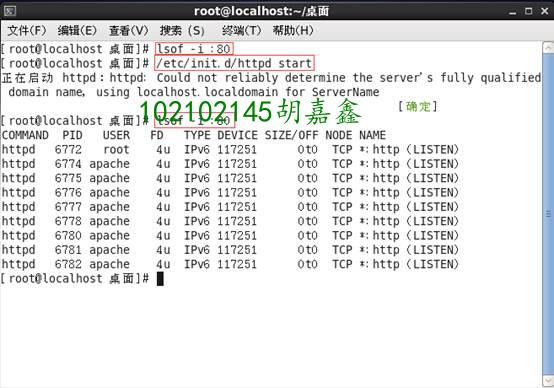
\includegraphics[width=0.40\textwidth]{2_9_1.jpeg}
  \end{center}
\end{figure}

此时防火墙 nat 表无规则。
\begin{figure}[H]
  \begin{center}
    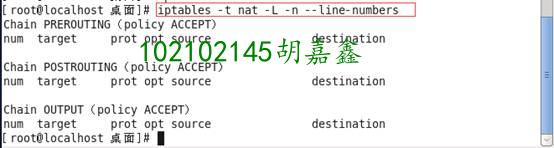
\includegraphics[width=0.40\textwidth]{2_9_2.jpeg}
  \end{center}
\end{figure}

此时在 Windows 7 上打开火狐浏览器,在地址栏输入
\texttt{http://192.168.1.200},打开的是防火墙 CentOS 6.5 上的
http 服务,即 Apache。
\begin{figure}[H]
  \begin{center}
    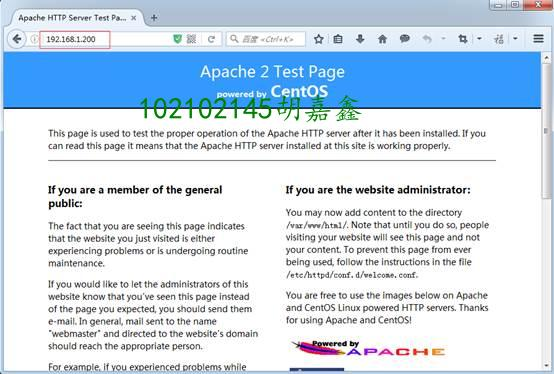
\includegraphics[width=0.40\textwidth]{2_9_3.jpeg}
  \end{center}
\end{figure}

在防火墙 CentOS6.5 的终端输入命令
\begin{minted}[bgcolor=bg,breaklines=true]{sh}
echo 1 > /proc/sys/net/ipv4/ip_forward
\end{minted}
开启防火墙数据包转发功能。
输入命令
\begin{minted}[bgcolor=bg,breaklines=true]{sh}
cat /proc/sys/net/ipv4/ip_forward
\end{minted}
进行查看。
此外,必须保证 \texttt{/etc/sysctl.conf} 文件中
\mintinline{sh}{net.ipv4.ip_forward} 的值为 1。
\begin{figure}[H]
  \begin{center}
    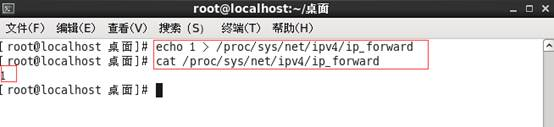
\includegraphics[width=0.40\textwidth]{2_9_4.jpeg}
  \end{center}
\end{figure}
\begin{figure}[H]
  \begin{center}
    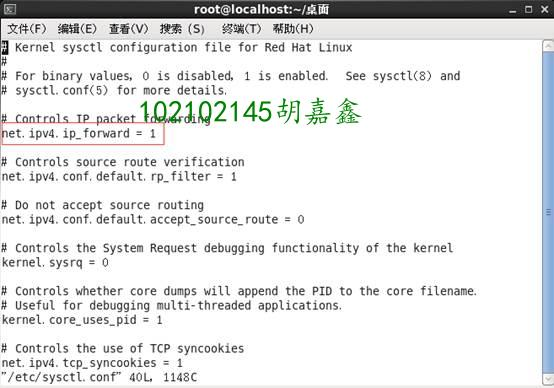
\includegraphics[width=0.40\textwidth]{2_9_5.jpeg}
  \end{center}
\end{figure}

在防火墙 CentOS 6.5 的终端输入如下命令,
\begin{minted}[bgcolor=bg,breaklines=true]{sh}
iptables -t nat -A PREROUTING -d 192.168.1.200 -p tcp --dport 80 -j DNAT --to-destination 20.0.0.2:80
iptables -t nat -A POSTROUTING -d 20.0.0.2 -p tcp --dport 80 -j SNAT --to-source 192.168.1.200
iptables -t nat -L -n --line-numbers
\end{minted}
将外部 IP 地址端口 \texttt{192.168.1.200:80} 映射到内部服务器
\texttt{20.0.0.2:80}。
\begin{figure}[H]
  \begin{center}
    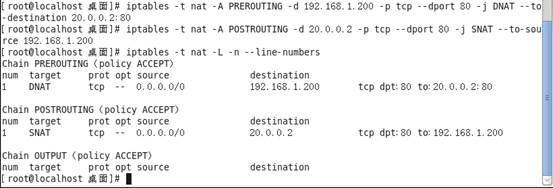
\includegraphics[width=0.40\textwidth]{2_9_6.jpeg}
  \end{center}
\end{figure}

在终端输入命令
\begin{minted}[bgcolor=bg,breaklines=true]{sh}
/etc/init.d/iptables save
\end{minted}
保存配置的防火墙规则。
输入命令
\begin{minted}[bgcolor=bg,breaklines=true]{sh}
cat /etc/sysconfig/iptables
\end{minted}
查看配置的防火墙规则。
\begin{figure}[H]
  \begin{center}
    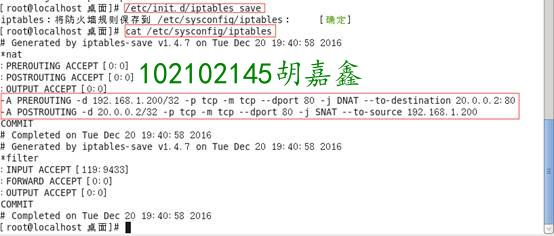
\includegraphics[width=0.40\textwidth]{2_9_7.jpeg}
  \end{center}
\end{figure}

此时在操作机Windows7上访问
\texttt{http://192.168.1.200}时访问的是内部服务器的网站
\texttt{http://20.0.0.2}。
\begin{figure}[H]
  \begin{center}
    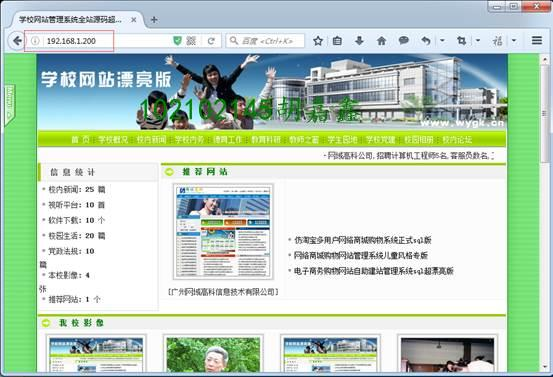
\includegraphics[width=0.40\textwidth]{2_9_8.jpeg}
  \end{center}
\end{figure}

%
\section{数据库安全}
%\subsection{实验目的-MSSQL攻击日志分析}
\begin{enumerate}
  \item 破解 SQL Server 2008 的 sa 密码
  \item 抓取破解过程中的数据包并分析
  \item 查看并分析 SQL Server 日志文件
\end{enumerate}
%
\subsection{实验原理}
TCP 协议与三次握手:
TCP(Transmission Control Protocol:传输控制协议) ,TCP 是主机对主机
层的传输控制协议,提供可靠的连接服务,采用三次握手确认建立一个连接。

位码即 tcp 标志位,有 6 种标示:
\begin{itemize}
  \item SYN(synchronous 建立联机)
  \item ACK(acknowledgement 确认)
  \item PSH(push 传送)
  \item FIN(finish 结束)
  \item RST(reset 重置)
  \item URG(urgent 紧急)
\end{itemize}
%
三次握手过程如下:
\begin{enumerate}
  \item 第一次握手:主机 A 发送位码为 $\texttt{SYN}=1$, 随机产生 SEQ number 的数据包到
    服务器,主机 B 由 $\texttt{SYN}=1$ 知道,A 要求建立联机;
  \item 第二次握手:主机 B 收到请求后要确认联机信息,
    向 A 发送 $\texttt{ACK number}=(\texttt{主机A的SEQ}+1),\texttt{SYN}=1,\texttt{ACK}=1$,
    随机产生 SEQ number 的包;
  \item 第三次握手:主机 A 收到后检查 ACK number 是否正确,
    即第一次发送的 $\texttt{SEQ number}+1$,
    以及位码 ack 是否为 1,若正确,
    主机 A 会再发送 $\texttt{ACK number}=(\texttt{主机B的SEQ}+1),\texttt{ACK}=1$,
    主机 B 收到后确认 SEQ 值与 $\texttt{ACK}=1$ 则连接建立成功。
\end{enumerate}
完成三次握手,主机 A 与主机 B 开始传送数据。
%
\subsection{实验环境}
\begin{itemize}
  \item Kali Linux:192.168.1.2 hydra
  \item Windows server 2003:192.168.1.3 SQL Server 2008 R2
\end{itemize}
%
\subsection{实验步骤}
\subsubsection{破解sa密码,并用wireshark抓取破解数据包}
在 Windows server 2003 上打开 wireshark,并抓取数据包。
\begin{figure}[H]
  \begin{center}
    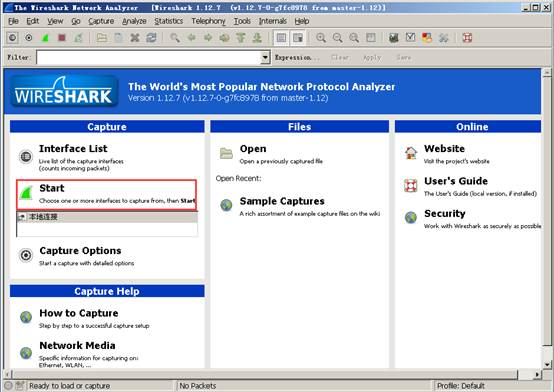
\includegraphics[width=0.40\textwidth]{2_10_1.jpeg}
  \end{center}
\end{figure}

在 Kali 上,查看用户名文件 \texttt{userlist.txt} 和
密码文件 \texttt{passlist.txt}。
\begin{figure}[H]
  \begin{center}
    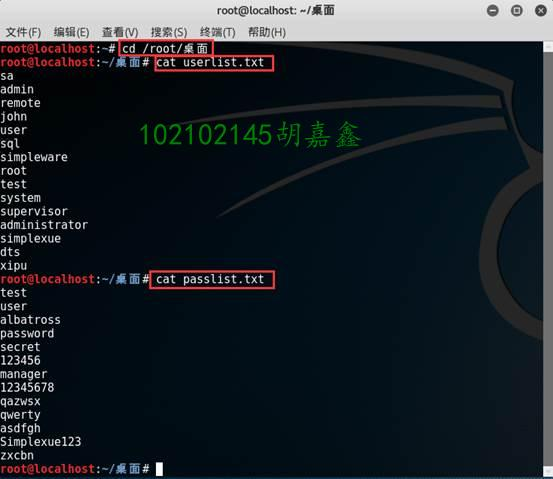
\includegraphics[width=0.40\textwidth]{2_10_2.jpeg}
  \end{center}
\end{figure}

在终端输入命令
\begin{minted}[bgcolor=bg,breaklines=true]{sh}
hydra -L userlist.txt -P passlist.txt 192.168.1.3 mssql -t 1
\end{minted}
开始破解 mssql,可以看到破解出 sa 的密码为 123456。
注意:
由于 hydra 的默认线程不是 1,为了更加便于后面数据包的分析,破解 mssql
时最好将线程数设为 1。
\begin{figure}[H]
  \begin{center}
    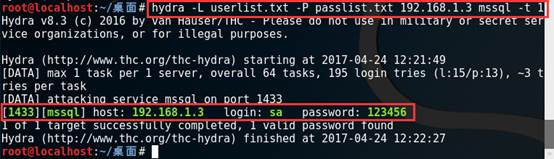
\includegraphics[width=0.40\textwidth]{2_10_3.jpeg}
  \end{center}
\end{figure}

返回 Windows server 2003,wireshark 停止抓包,
过滤端口为 1433 的数据包。
\begin{figure}[H]
  \begin{center}
    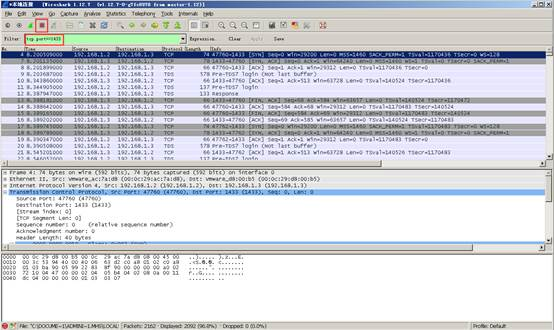
\includegraphics[width=0.40\textwidth]{2_10_4.jpeg}
  \end{center}
\end{figure}
%
\subsubsection{分析抓取的数据包,理解 mssql 破解过程}
首先查看第一个数据包,源地址为 \texttt{192.168.1.2},源端口为 \texttt{47366},
目的地址为 \texttt{192.168.1.3},目的端口为 \texttt{1433},
TCP 序号为 SYN,且置为 1,
表示客户端 \texttt{192.168.1.2} 向服务器 \texttt{192.168.1.3} 发送了一个连接请求报文。
\begin{figure}[H]
  \begin{center}
    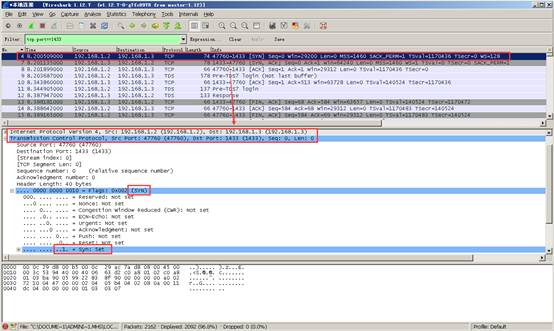
\includegraphics[width=0.40\textwidth]{2_10_5.jpeg}
  \end{center}
\end{figure}

再查看第二个数据包,\texttt{192.168.1.3} 收到请求后确认联机信息,
向 \texttt{192.168.1.2} 发送数据包,SYN 置为 1,ACK 也置为 1。
\begin{figure}[H]
  \begin{center}
    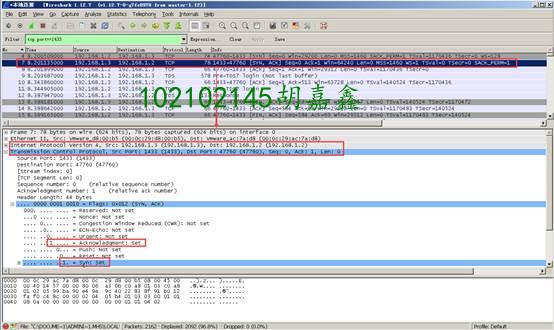
\includegraphics[width=0.40\textwidth]{2_10_6.jpeg}
  \end{center}
\end{figure}

查看第三个数据包,主机 \texttt{192.168.1.2} 收到数据包后检查无误,
向 \texttt{192.168.1.3} 发送数据包,ACK 置为 1,
至此三次握手完毕,连接建立,后面就可以开始传输数据了。
\begin{figure}[H]
  \begin{center}
    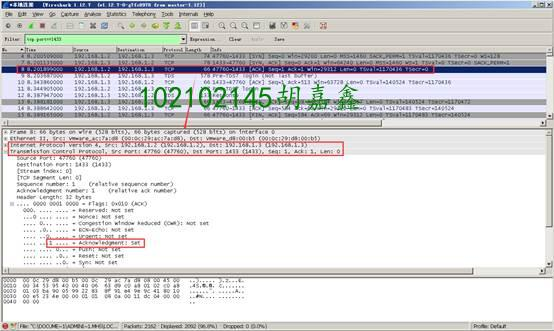
\includegraphics[width=0.40\textwidth]{2_10_7.jpeg}
  \end{center}
\end{figure}

查看第四个数据包,可以看到传输的数据,其中包括了用户名 sa 和密码 test,
表明正在破解 mssql。
\begin{figure}[H]
  \begin{center}
    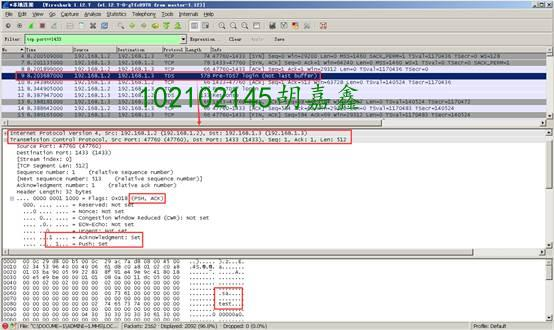
\includegraphics[width=0.40\textwidth]{2_10_8.jpeg}
  \end{center}
\end{figure}

查看 response,可以看到为 false,说明连接不成功,即用户名或者密码错
误。之后则是连接的结束过程。
\begin{figure}[H]
  \begin{center}
    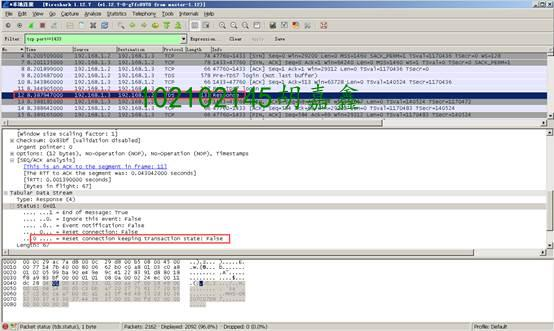
\includegraphics[width=0.40\textwidth]{2_10_9.jpeg}
  \end{center}
\end{figure}

通过分析抓取的数据包,我们可以得知,重复的过程实际上也就是 mssql 破
解的过程。
\begin{figure}[H]
  \begin{center}
    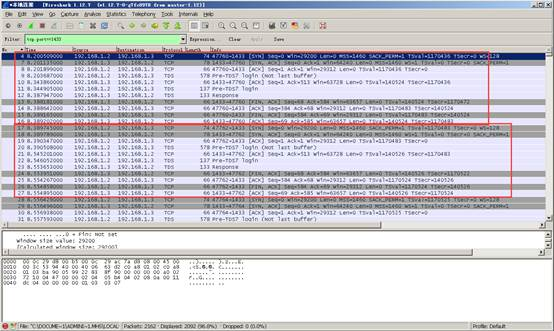
\includegraphics[width=0.40\textwidth]{2_10_10.jpeg}
  \end{center}
\end{figure}

我们找到破解出来的 sa 密码 123456 对应的数据包,并查看其 response 数
据包,发现与其它 response 数据包相比,多了一些数据,说明 sa 的密码很
有可能是 123456,实际上也的确如此。
\begin{figure}[H]
  \begin{center}
    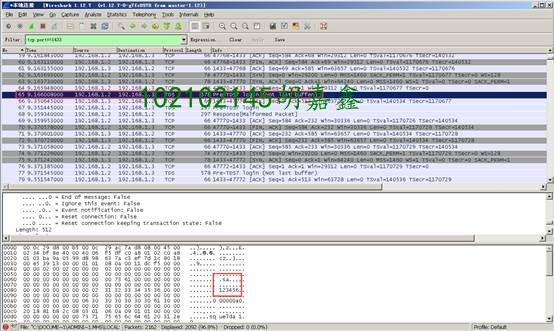
\includegraphics[width=0.40\textwidth]{2_10_11.jpeg}
  \end{center}
\end{figure}
\begin{figure}[H]
  \begin{center}
    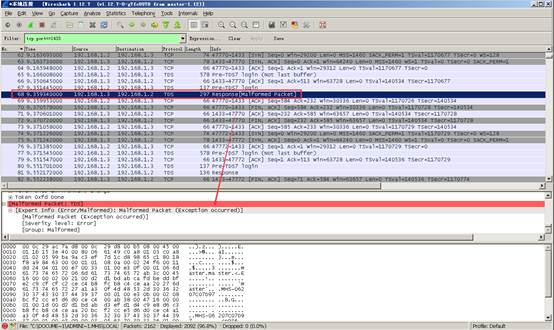
\includegraphics[width=0.40\textwidth]{2_10_12.jpeg}
  \end{center}
\end{figure}
%
\subsubsection{查看 mssql 日志}
单击``开始'' $ \rightarrow $ ``所有程序''
$ \rightarrow $ ``Microsoft SQL Server 2008 R2`` $ \rightarrow $
``SQL Server Management Studio''。
\begin{figure}[H]
  \begin{center}
    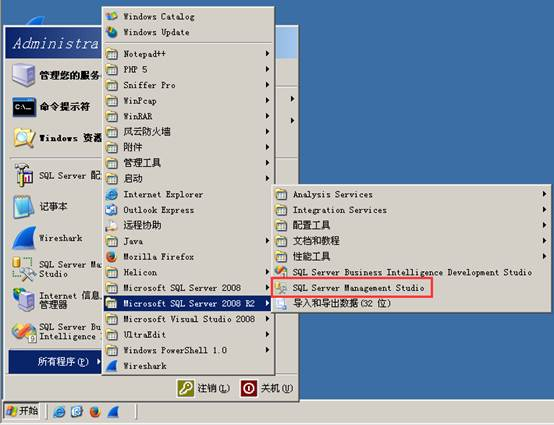
\includegraphics[width=0.40\textwidth]{2_10_13.jpeg}
  \end{center}
\end{figure}

以``Windows 身份认证''方式进行登录
(也可用前面破解出来的 \texttt{sa/123456} 进行登录,
不过登录方式要选择 SQL Server 身份认证)。
\begin{figure}[H]
  \begin{center}
    \includegraphics[width=0.40\textwidth]{2_10_14.jpeg}
  \end{center}
\end{figure}

展开``管理'' $ \rightarrow $ ``SQL Server 日志'',双击当前日志。
\begin{figure}[H]
  \begin{center}
    \includegraphics[width=0.40\textwidth]{2_10_15.jpeg}
  \end{center}
\end{figure}

在打开的日志文件查看器中查看到的 SQL Server 日志信息中,可以看到前
面破解过程中尝试登录的情况,例如以 xipu 用户名进行登录时,提示``找
不到与所提供的名称相匹配的登录名'',说明登录名中没有 xipu。其中,前
两条日志记录是使用 Windows 身份认证进行登录的信息。看到这么多短时间
内登录失败的日志信息,我们就可以得知数据库遭受了攻击,需要采取一定
的手段进行防御。
\begin{figure}[H]
  \begin{center}
    \includegraphics[width=0.40\textwidth]{2_10_16.jpeg}
  \end{center}
\end{figure}

使用 sa 尝试进行登录时,提示``密码与所提供的登录名不匹配'',说明 sa
是一个登录名。在使用 sa 破解的过程中,有两条信息与使用 Windows 身份
认证进行登录时的日志信息很相似,我们可以猜测该记录对应的 sa 密码是
正确的,实际上也的确如此。
\begin{figure}[H]
  \begin{center}
    \includegraphics[width=0.40\textwidth]{2_10_17.jpeg}
  \end{center}
\end{figure}

%\subsection{实验目的-了解 MySQL 日志}
了解 MySQL 日志.
%
\subsection{实验原理}
日志是 mysql 数据库的重要组成部分。日志文件中记录着 mysql 数据库运行期间发生的变化,
也就是说用来记录 mysql 数据库的客户端连接状况、SQL 语句的执行情况和错误信息等。当
数据库遭到意外的损坏时,可以通过日志查看文件出错的原因,并且可以通过日志文件进
行数据恢复。
%
\subsection{实验环境}
CentOS6.5:192.168.1.3 MySQL
%
\subsection{实验步骤}
\subsubsection{MySQL 日志介绍}
MySQL 有以下几种日志:
\begin{itemize}
  \item 错误日志:log-err
  \item 查询日志:log
  \item 慢查询日志:log-slow-queries
  \item 二进制日志:log-bin
  \item 更新日志:log-update
\end{itemize}
%
错误日志:记录 MySQL Server 启动和关闭的详细信息、以及运行过程中较为严重的警告和
错误信息,修改错误日志的地址可以在\texttt{/etc/my.cnf} 中添加
\begin{minted}[bgcolor=bg,breaklines=true]{sh}
-log-error = [filename]
\end{minted}
来设置 mysql 错误日志,在 mysql 中是默认开启错误日志的。
%\begin{figure}[H]
  %\begin{center}
    %\includegraphics[width=0.50\textwidth]{}
  %\end{center}
%\end{figure}
%\begin{figure}[H]
  %\begin{center}
    %\includegraphics[width=0.50\textwidth]{}
  %\end{center}
%\end{figure}

查询日志:记录 mysql 的日常日志,包括查询、修改、更新等的每条 SQL 语句信息。
使用
\begin{minted}[bgcolor=bg,breaklines=true]{sh}
show global variables like '%genera%';
\end{minted}
查看 mysql 是否启用了查询日志。可以看到此时的查询日志是关闭的。
%\begin{figure}[H]
  %\begin{center}
    %\includegraphics[width=0.50\textwidth]{}
  %\end{center}
%\end{figure}

mysql 打开 general log 日志后,所有的查询语句都可以在 general log 文件中输出,
如果打开,文件会非常大,建议调试的时候打开,平时关闭。
查询日志的输出文件可以在
\texttt{/etc/my.cnf} 中添加
\begin{minted}[bgcolor=bg,breaklines=true]{sh}
general-log-file = [filename]
\end{minted}
来开启,也可以使用命令
\begin{minted}[bgcolor=bg,breaklines=true]{sh}
set global general_log = on;
set global general_log = off;
\end{minted}
在 mysql 中打开和关闭。
%\begin{figure}[H]
  %\begin{center}
    %\includegraphics[width=0.50\textwidth]{}
  %\end{center}
%\end{figure}

开启查询日志并新建一个名为 simpleware 的数据库。再关闭查询日志,可以看到在查询日
志中记录了创建数据库 simpleware 和关闭查询日志的 SQL 语句。
%\begin{figure}[H]
  %\begin{center}
    %\includegraphics[width=0.50\textwidth]{}
  %\end{center}
%\end{figure}
%\begin{figure}[H]
  %\begin{center}
    %\includegraphics[width=0.50\textwidth]{}
  %\end{center}
%\end{figure}

慢查询日志:慢查询日志中记录的是执行时间较长的 query,
可以设一个阀值、将运行时间超过该值的所有 SQL 语句都记录到慢查询日志文件中。
该阀值可以通过参数 \texttt{long\_query\_time} 来设置,默认是 10 秒。
注意:对于运行时间正好等于 \texttt{long\_query\_time} 的情况并不会
被记录,因为在源代码里是判断大于 \texttt{long\_query\_time},而非大于等于。

可以输入命令
\begin{minted}[bgcolor=bg,breaklines=true]{sh}
show variables like '%slow%';
\end{minted}
查看慢查询日志功能是否开启,可以看到此时慢查询日志功能并未开启。
%\begin{figure}[H]
  %\begin{center}
    %\includegraphics[width=0.50\textwidth]{}
  %\end{center}
%\end{figure}

可使用命令
\begin{minted}[bgcolor=bg,breaklines=true]{sh}
set global slow_query_log = on;
set global slow_query_log = off;
\end{minted}
开启或关闭慢查询日志功能。
%\begin{figure}[H]
  %\begin{center}
    %\includegraphics[width=0.50\textwidth]{}
  %\end{center}
%\end{figure}

二进制日志文件:记录与修改有关的信息,影响数据潜在的内容的信息,
二进制日志也叫复制日志,默认在数据目录下,
专门查看 mysql 二进制日志文件的命令是 \texttt{mysqlbinlog}。

MySQL 记录二进制日志的格式有三种:
\begin{enumerate}
  \item 基于语句:statement,每一条会修改数据的 sql 都会记录到 master 的 binlog 中,
    slave 在复制的时候,sql 进程会解析成和原来 master 端相同的
    sql 再执行。
  \item 基于行的:row,日志中会记录成每一行数据被修改的形式,
    然后在 slave 端再对相同的数据
    进行修改,只记录要修改的数据,只有 value,
    不会有 sql 多表关联的情况。
  \item 混合模式:mixed,由 MySQL 自己判断以什么方式记录日志,
    MySQL 会根据执行的每一条具体
    的 SQL 语句来区分对待记录的日志形式,
    也就是在 statement 和 row 之间选择一种。
\end{enumerate}

使用命令
\begin{minted}[bgcolor=bg,breaklines=true]{sh}
show variables like '%log_bin%';
\end{minted}
查看mysql 二进制日志文件的配置情况,
log\_bin 用于设定是否启用二进制日志功能,
可以看到此时二进制日志功能未开启。
%\begin{figure}[H]
  %\begin{center}
    %\includegraphics[width=0.50\textwidth]{}
  %\end{center}
%\end{figure}

%\subsection{实验目的-MySQL 日志}
了解 MySQL 日志.
%
\subsection{实验原理}
日志是 mysql 数据库的重要组成部分。日志文件中记录着 mysql 数据库运行期间发生的变化,
也就是说用来记录 mysql 数据库的客户端连接状况、SQL 语句的执行情况和错误信息等。当
数据库遭到意外的损坏时,可以通过日志查看文件出错的原因,并且可以通过日志文件进
行数据恢复。
%
\subsection{实验环境}
Kali Linux:192.168.1.2 hydra
CentOS6.5:192.168.1.3 MySQL
%
\subsection{实验步骤}
\subsubsection{破解mysql的root密码,并抓取破解数据包}
在实验开始前先开启 CentOS6.5 上的通用日志。
在 kali linux 的终端中输入命令``wireshark'',回车,打开 wireshark。
%\begin{figure}[H]
  %\begin{center}
    %\includegraphics[width=0.50\textwidth]{}
  %\end{center}
%\end{figure}

在打开的 wireshark 中选择要监听的网卡,单击``开始捕获分组''按钮,
开始进行抓包。
%\begin{figure}[H]
  %\begin{center}
    %\includegraphics[width=0.50\textwidth]{}
  %\end{center}
%\end{figure}

重新打开一个终端,输入命令
\begin{minted}[bgcolor=bg,breaklines=true]{sh}
cd /root/桌面
cat userlist.txt
cat passlist.txt
\end{minted}
查看用户名文件和密码文件。
%\begin{figure}[H]
  %\begin{center}
    %\includegraphics[width=0.50\textwidth]{}
  %\end{center}
%\end{figure}

在终端输入命令
\begin{minted}[bgcolor=bg,breaklines=true]{sh}
hydra -L userlist.txt -P passlist.txt 192.168.1.3 mysql -t 1
\end{minted}
开始破解 mysql。
这里为了便于后面的数据包分析,将线程数设置为 1。
%\begin{figure}[H]
  %\begin{center}
    %\includegraphics[width=0.50\textwidth]{}
  %\end{center}
%\end{figure}

在破解的过程中发现耗时估计会很长,请耐心等待。这里我们为了便于分析,
新建并简化用户名文件和密码文件。
%\begin{figure}[H]
  %\begin{center}
    %\includegraphics[width=0.50\textwidth]{}
  %\end{center}
%\end{figure}

重新开始抓包,在终端输入命令
\begin{minted}[bgcolor=bg,breaklines=true]{sh}
hydra -L user.txt -P pass.txt 192.168.1.3 mysql -t 1
\end{minted}
开始破解 mysql。
%\begin{figure}[H]
  %\begin{center}
    %\includegraphics[width=0.50\textwidth]{}
  %\end{center}
%\end{figure}

wireshark 停止抓包,过滤端口为 3306 的数据包。
%\begin{figure}[H]
  %\begin{center}
    %\includegraphics[width=0.50\textwidth]{}
  %\end{center}
%\end{figure}
%
\subsubsection{分析抓取的数据包,理解 mysql 破解过程}
通过观察 wireshark 抓取的数据包可知,wireshark 已经对抓取的数据包使用
``[''的符号对连接建立、传输数据、断开连接的过程进行了标识。
%\begin{figure}[H]
  %\begin{center}
    %\includegraphics[width=0.50\textwidth]{}
  %\end{center}
%\end{figure}

下面我们对其中一个过程的数包进行分析。首先查看第一个数据包,
源地址为 \texttt{192.168.1.2},源端口为 \texttt{44578},目的地址为\texttt{192.168.1.3},
目的端口为 \texttt{3306},TCP 序号为 SYN,且置为 $1$,
表示客户端 \texttt{192.168.1.2} 向服务器 \texttt{192.168.1.3} 发送了一个连接请求报文。
%\begin{figure}[H]
  %\begin{center}
    %\includegraphics[width=0.50\textwidth]{}
  %\end{center}
%\end{figure}

再查看第二个数据包,
\texttt{192.168.1.3} 收到请求后确认联机信息,向 \texttt{192.168.1.2} 发送数据包,
SYN 置为 $1$,ACK 也置为 $1$。
%\begin{figure}[H]
  %\begin{center}
    %\includegraphics[width=0.50\textwidth]{}
  %\end{center}
%\end{figure}

查看第三个数据包,主机 \texttt{192.168.1.2} 收到数据包后检查无误,
向 \texttt{192.168.1.3} 发送数据包,
ACK 置为 $1$,至此三次握手完毕,连接建立,后面就可以开始传输数据了。
%\begin{figure}[H]
  %\begin{center}
    %\includegraphics[width=0.50\textwidth]{}
  %\end{center}
%\end{figure}

从这个数据包信息可知,mysql 的版本为 \texttt{5.1.73}。
%\begin{figure}[H]
  %\begin{center}
    %\includegraphics[width=0.50\textwidth]{}
  %\end{center}
%\end{figure}

查看这个数据包,可以看到传输的数据,即 mysql 登录信息,用户名为 sql,
表明正在破解 mysql。
由上一步骤的数据包信息可
知 mysql 对密码进行了加盐。
%\begin{figure}[H]
  %\begin{center}
    %\includegraphics[width=0.50\textwidth]{}
  %\end{center}
%\end{figure}

查看 Response,可以看到为 Error,说明连接不成功,即用户名或者密码错误。
之后则是连接的结束过程。
%\begin{figure}[H]
  %\begin{center}
    %\includegraphics[width=0.50\textwidth]{}
  %\end{center}
%\end{figure}

我们找到破解出来的 root 密码对应的数据包,
并查看其 response 数据包,发现与其它 response 数据包相比,
为 OK。
%\begin{figure}[H]
  %\begin{center}
    %\includegraphics[width=0.50\textwidth]{}
  %\end{center}
%\end{figure}
%\begin{figure}[H]
  %\begin{center}
    %\includegraphics[width=0.50\textwidth]{}
  %\end{center}
%\end{figure}
%
\subsubsection{查看 mysql 通用日志}
在 CentOS6.5 上打开终端,输入命令
\begin{minted}[bgcolor=bg,breaklines=true]{sh}
service mysqld start
mysql -u root -p
# 密码 123456
\end{minted}
%\begin{figure}[H]
  %\begin{center}
    %\includegraphics[width=0.50\textwidth]{}
  %\end{center}
%\end{figure}

在 mysql 中输入命令
\begin{minted}[bgcolor=bg,breaklines=true]{sh}
set global general_log = on;
\end{minted}
开启通用日志,再输入命令
\begin{minted}[bgcolor=bg,breaklines=true]{sh}
show global variables like '%genera%';
\end{minted}
进行查看,可以看到通用日志已开启。
%\begin{figure}[H]
  %\begin{center}
    %\includegraphics[width=0.50\textwidth]{}
  %\end{center}
%\end{figure}

在终端输入命令
\begin{minted}[bgcolor=bg,breaklines=true]{sh}
cat /var/run/mysqld/mysqld.log
\end{minted}
查看到前面破解过程的 mysql 登录
信息。
%\begin{figure}[H]
  %\begin{center}
    %\includegraphics[width=0.50\textwidth]{}
  %\end{center}
%\end{figure}

%\subsection{实验目的-了解oracle日志文件}
了解 oracle 日志文件.
%
\subsection{实验原理}
\begin{enumerate}
  \item 用户对 oracle 数据库的一切操作都记录在数据库的日志文件中,通过日志文件可以查看用户
    对数据库进行了哪些操作
  \item oracle 分三大类:
    \begin{itemize}
      \item Alert log files(告警日志)、
      \item Trace files (跟踪日志:用户和进程)
      \item redo log(重做日志:记录数据库的更改)。
    \end{itemize}
\end{enumerate}
%
\subsection{实验环境}
Windows server 2008 R2:192.168.1.3 oracle 11g
%
\subsection{实验步骤}
\subsubsection{告警日志}
告警日志文件是一类特殊的跟踪文件(trace file)。
告警日志文件命名一般为 \texttt{alert\_<SID>.log},
其中 \texttt{SID} 为 ORACLE 数据库实例名称。
数据库告警日志是按时间顺序记录 message 和错误信息。

在 ORACLE 10g 中,\texttt{BACKGROUND\_DUMP\_DEST} 参数确定了告警日志的位置,
但是告警日志的文件名无法修改。
\texttt{BACKGROUND\_DUMP\_DEST} 参数是动态的。告警日志以及所有后台跟踪文件都
会被写至 \texttt{BACKGROUND\_DUMP\_DEST} 参数所指定的目录。

在 ORACLE 11g 以及 ORACLE 12c 中,告警日志文件的位置有了变化。
主要是因为引入了 ADR
(Automatic Diagnostic Repository:一个存放数据库诊断日志、跟踪文件的目录),
关于 ADR 对应的目录位置可以通过查看 v\$diag\_info 系统视图。

在 cmd 中输入命令
\begin{minted}[bgcolor=bg,breaklines=true]{sh}
sqlplus sys/Simplexue123 as sysdba
\end{minted}
登录 oracle 数据库。
%\begin{figure}[H]
  %\begin{center}
    %\includegraphics[width=0.50\textwidth]{}
  %\end{center}
%\end{figure}

在 SQL 中输入命令
\begin{minted}[bgcolor=bg,breaklines=true]{sql}
select * from v$diag_info;
\end{minted}
查看 ADR 对应的目录位置,可以看到 Diag Trace 对应的目录为文本格式的告警日志文件所在的目录,
而 Diag Alert 对应的目录为 XML 格式的警告日志(对应为 log.xml)。
%\begin{figure}[H]
  %\begin{center}
    %\includegraphics[width=0.50\textwidth]{}
  %\end{center}
%\end{figure}
%\begin{figure}[H]
  %\begin{center}
    %\includegraphics[width=0.50\textwidth]{}
  %\end{center}
%\end{figure}
%\begin{figure}[H]
  %\begin{center}
    %\includegraphics[width=0.50\textwidth]{}
  %\end{center}
%\end{figure}

告警日志包含了下面一些内容的信息。像一些 ORA 错误,对于监控数据库有极其重要的作用。
\begin{enumerate}
  \item 所有的内部错误(ORA-600)信息,块损坏错误(ORA-1578)信息,以及死锁错误(ORA-60)
    信息等。
  \item 管理操作,例 CREATE、ALTER、DROP 语句等,以及数据库启动、关闭以及日志归档的一些
    信息。包括以下两类:
    \begin{itemize}
      \item 涉及物理结构的所有操作:例如创建、删除、重命名数据文件与联机重做日志文件的
        \texttt{ALTER DATABASE} 命令,此外还涉及重新分配数据文件大小以及将数据文件联机与脱机的操作。
      \item 表空间操作:例如 \texttt{DROP} 与 \texttt{CREATE} 命令,
        此外还包括为了进行用户管理的备份而将表空间置入和取出热备份模式的操作
    \end{itemize}
  \item 与共享服务器或调度进程相关功能的消息和错误信息。
  \item 物化视图的自动刷新过程中出现的错误。
  \item 动态参数的修改信息。
\end{enumerate}

既然告警日志如此重要,而我们也不可能随时手工去查看告警日志文件,那么我们就必须监
控告警日志,那么监控告警日志有哪些方案呢?有以下 3 种方案:
\begin{itemize}
  \item 在 ORACLE 10g,可以将告警日志文件信息读入全局临时表,然后就可以定制一些 SQL 语句查
    询告警日志的信息。但这个方案有几个不足之处,一是如果数据库宕机了的情况下,是无
    法获取这些错误信息的,因此有些特定场景不适用。二是日志文件比较大的时候,监控告
    警日志信息比较频繁的时候,会产生不必要的 IO 操作。
  \item 通过外部表来查看告警日志文件的内容,相当的方便,与方案一一样也是使用定制
    SQL 语句来查询错误信息。
  \item 将告警日志进行归档。告警日志文件如果不加管理的话,那么文件会持续增长,有
    时候文件会变得非常大,不利于读写。一般建议将告警日志按天归档,归档文件保留三个
    月(视情况而定),可通过编写脚本来进行归档。
\end{itemize}
%
\subsubsection{跟踪日志}
跟踪文件(trace file)的作用,通常是一个服务器进程对某种异常错误条件做出响应时创
建的诊断文件。一个 sql 发到数据库,肯定会有一个
``接收请求 $\rightarrow$ 数据处理 $\rightarrow$ 返回应答''
的过程。那么就需要不同的进程来执行相应的步骤。如果进程在执行过程中发生错误,
那么就会记录到跟踪文件中。

在创建数据库的过程中遇到的错误,可以通过查找 Oracle 数据库的告警日志文件获得,
在某些情况下,还会有详细的跟踪文件生成,这些文件的位置,
在 Oracle 11g 之前,由 \texttt{*dump} 参数指定,
告警日志文件 \texttt{alert\_<ORACLE\_SID>.log} 的位置由
参数 \texttt{background\_dump\_dest} 定义。

跟踪文件的查看命令为
\begin{minted}[bgcolor=bg,breaklines=true]{sql}
show parameter SQL_TRACE;
\end{minted}
如果结果为 FALSE,
可使用命令
\begin{minted}[bgcolor=bg,breaklines=true]{sql}
alter system set SQL_TRACE = TRUE SCOPE = both;
\end{minted}
来设置打开,
使用命令
\begin{minted}[bgcolor=bg,breaklines=true]{sql}
alter system set SQL_TRACE = FALSE;
\end{minted}
来进行关闭。
%\begin{figure}[H]
  %\begin{center}
    %\includegraphics[width=0.50\textwidth]{}
  %\end{center}
%\end{figure}

在 SQL 中输入命令
\begin{minted}[bgcolor=bg,breaklines=true]{sql}
show parameter DUMP_DEST;
\end{minted}
查看跟踪文件位置,
会看到有三个跟踪文件目录。
%\begin{figure}[H]
  %\begin{center}
    %\includegraphics[width=0.50\textwidth]{}
  %\end{center}
%\end{figure}

其中,\texttt{background\_dump\_dest} 为后台转储,
\texttt{core\_dump\_dest} 为内核转储,
\texttt{user\_dump\_dest} 为用户转储,一般而言,
我们只对后台和用户转储目标感兴趣。

在 SQL 中输入命令
\begin{minted}[bgcolor=bg,breaklines=true]{sql}
show parameter background_dump_dest;
\end{minted}
查看后台转储跟踪日志文件的路径。
%\begin{figure}[H]
  %\begin{center}
    %\includegraphics[width=0.50\textwidth]{}
  %\end{center}
%\end{figure}

可知跟踪日志文件所在的路径,
可以在该路径下,找到日志文件。
跟踪文件名形如:\texttt{orcl\_cjq0\_2348.trc}(SID 名+进程名+ 进程 ID)。
%\begin{figure}[H]
  %\begin{center}
    %\includegraphics[width=0.50\textwidth]{}
  %\end{center}
%\end{figure}
%
\subsubsection{重做日志}
重做日志分为在线重做日志和归档重做日志。
重做日志的简单原理:
在数据更新操作 commit 前,将更改的 SQL 脚本写入重做日志。
主要用于数据库的增量备份和增量恢复。
重做日志直接对应于硬盘的重做日志文件(有在线和归档二种),重做日志文件以组(Group)
的形式组织,一个重做日志组包含一个或者多个日志文件。

online Redo log files:在线重做日志,又称联机重做日志,指 Oracle 以 SQL 脚本的形
式 实时记录数据库的数据更新,换句话说,实时保存已执行的 SQL 脚本到在线日志文件中
(按特定的格式)。

对于在线重做日志,Oracle 11g 默认对于每个数据库实例,建立 3 个在线日志组,每组一个
日志文件,文件名称为 REDO01.LOG,REDO02.LOG 和 REDO03.LOG。(用户可以通过视图操作
添加/修改/删除日志组和日志文件来自定义在线重做日志)

每组内的日志文件的内容完全相同,且保存在不同的位置,用于磁盘日志镜像,以做多次备
份提高安全性。默认情况这 3 组通常只有一组处于活动状态,不断地同步写入已操作的脚
本,当日志文件写满时(达到指定的空间配额),如果当前数据库处于归档模式,则将在
线日志归档到硬盘,成为归档日志;若当前数据库处于非归档模式,则不进行归档操作,
而当前在线日志的内容会被下一次重新写入覆盖而无法保存。因此,通常数据库在运行时,
是处于归档模式下的,以保存数据更新的日志。

当前归档日志组写满后,Oracle 会切换到下一日志组,继续写入,就这样循环切换;当处于
归档模式下,切换至原已写满的日志组,若该日志组归档完毕则覆盖写入,若没有则只能
使用日志缓冲区,等待归档完毕之后才能覆盖写入。当然,处于非归档模式下是直接覆盖
写入的。

Oracle 提供了 2 个视图用于维护在线重做日志:V\$LOG 和 V\$LOGFILE,
我们可以通过这两个视图查看和修改在线日志。

在 SQL 中输入命令
\begin{minted}[bgcolor=bg,breaklines=true]{sh}
SELECT * FROM v$log;
\end{minted}
通过 v\$log 视图查询在线日志的总体信息。
%\begin{figure}[H]
  %\begin{center}
    %\includegraphics[width=0.50\textwidth]{}
  %\end{center}
%\end{figure}

为了便于查看,复制到 txt 文件整理后的在线日志的总体信息如下。
%\begin{figure}[H]
  %\begin{center}
    %\includegraphics[width=0.50\textwidth]{}
  %\end{center}
%\end{figure}

在 SQL 中输入命令
\begin{minted}[bgcolor=bg,breaklines=true]{sql}
SELECT * FROM v$logfile ORDER BY group#;
\end{minted}
通过 v\$logfile 视图查询在线日志文件信息。
%\begin{figure}[H]
  %\begin{center}
    %\includegraphics[width=0.50\textwidth]{}
  %\end{center}
%\end{figure}

为了便于查看,复制到 txt 文件整理后的在线日志文件信息如下。
%\begin{figure}[H]
  %\begin{center}
    %\includegraphics[width=0.50\textwidth]{}
  %\end{center}
%\end{figure}

此外可以通过 ALTER、DATABASE、ADD、DELETE 等命令增加、
修改或删除在线日志或日志组.

Archive Redo log files:归档重做日志,简称归档日志,
指当条件满足时,Oracle 将在线重做日志以文件形式保存到硬盘(持久化)。

所谓的归档,就是指将在线日志进行归档、持久化到成固定的文件到硬盘,便于以后的恢
复和查询。当然,前提条件是数据库要处于归档模式。

Oracle 11g 默认是为归档日志设定 2 个归档位置,
这 2 个归档位置的的归档日志的内容完全一致,但文件名不同。


% [1] 中 国 互 联 网 协 会 2006 年 第 一 次 反 垃 圾 邮 件 调 查 结 果
% [EOL].http://www.anti-spam.cnlShowArticle.php?id=2713
% [2] 曹麒麟,张千里.垃圾邮件与反垃圾邮件技术[M].北京:人民邮电出版社,2003.
% [3] 罗改龙.基于 SPI 的防火墙的研究与实现[硕士学位论文].武汉:武汉理工大学,2007
% [4] 周茜,赵明生.中文文本分类中的特征选择研究[J].中文信息学报,2003,Vol.18 No.3
\end{document}
